%% abtex2-modelo-trabalho-academico.tex, v-1.9.3 laurocesar
%% Copyright 2012-2015 by abnTeX2 group at http://abntex2.googlecode.com/
%% This work may be distributed and/or modified under the
%% conditions of the LaTeX Project Public License, either version 1.3
%% of this license or (at your option) any later version.
%% The latest version of this license is in
%%   http://www.latex-project.org/lppl.txt
%% and version 1.3 or later is part of all distributions of LaTeX
%% version 2005/12/01 or later.
%%
%% This work has the LPPL maintenance status `maintained'.
%%
%% The Current Maintainer of this work is the abnTeX2 team, led
%% by Lauro César Araujo. Further information are available on
%% http://abntex2.googlecode.com/
%%
%% This work consists of the files abntex2-modelo-trabalho-academico.tex,
%% abntex2-modelo-include-comandos and abntex2-modelo-references.bib
%%

% ------------------------------------------------------------------------
% ------------------------------------------------------------------------
% abnTeX2: Modelo de Trabalho Academico (tese de doutorado, dissertacao de
% mestrado e trabalhos monograficos em geral) em conformidade com
% ABNT NBR 14724:2011: Informacao e documentacao - Trabalhos academicos -
% Apresentacao
% ------------------------------------------------------------------------
% ------------------------------------------------------------------------

\documentclass{ufscThesis}
	% -- opções da classe memoir --
	% 12pt,				% tamanho da fonte
	% openright,			% capítulos começam em pág ímpar (insere página vazia caso preciso)
	% twoside,			% para impressão em verso e anverso. Oposto a oneside
	% a4paper,			% tamanho do papel.
	% -- opções da classe abntex2 --
	%chapter=TITLE,		% títulos de capítulos convertidos em letras maiúsculas
	%section=TITLE,		% títulos de seções convertidos em letras maiúsculas
	%subsection=TITLE,	% títulos de subseções convertidos em letras maiúsculas
	%subsubsection=TITLE,% títulos de subsubseções convertidos em letras maiúsculas
	% -- opções do pacote babel --
	% english,			% idioma adicional para hifenização
	% brazil				% o último idioma é o principal do documento

% ---
% Pacotes básicos
% ---
% \usepackage{times}				% Usa a fonte Latin Modern			lmodern
% \usepackage{mathptmx}
% \usepackage{pslatex}
% \usepackage[T1]{fontenc}		% Selecao de codigos de fonte.
% \usepackage{sbc-template}
% \usepackage[utf8]{inputenc}		% Codificacao do documento (conversão automática dos acentos)
% \usepackage{fontspec}		% Selecao de codigos de fonte.
% \usepackage[utf8]{inputenc}		% Codificacao do documento (conversão automática dos acentos)
% \setmainfont{Times New Roman}
% \usepackage{lastpage}			% Usado pela Ficha catalográfica
% \usepackage{indentfirst}		% Indenta o primeiro parágrafo de cada seção.
% \usepackage{color}				% Controle das cores
\usepackage{graphicx}			% Inclusão de gráficos
% \usepackage{microtype} 			% para melhorias de justificação
% \usepackage{biblatex}
\usepackage{chngcntr}
\usepackage{xspace}
\usepackage{pgfgantt}
\usepackage{adjustbox}
\usepackage[labelsep=endash]{caption}
% pacotes adicionados
% \usepackage{amsmath}
% \usepackage{amssymb,amsfonts,amsthm}
\usepackage{url}
\usepackage[acronym,nopostdot,nonumberlist]{glossaries}

% \usepackage{color}
% \usepackage{caption}
% Code Snippets
\usepackage{listings}
\renewcommand{\lstlistingname}{Código}
\lstset{
    basicstyle=\scriptsize\ttfamily,
	numbers=left,
	stepnumber=1,
	numbersep=-0.75em,
	keywordstyle=\color{blue},
	commentstyle=\color{black},
	stringstyle=\color{black},
    numberstyle=\scriptsize\ttfamily\color{black},
	frame=single,
	tabsize=2,
	float,
	language=C++,
	captionpos=t,
	showstringspaces=false,
	backgroundcolor=\color{white},
	morekeywords = {Array2D, __parallel__, Mask2D, Stencil2D},
	emph={
		pragma,
		omp,
		parallel,
		reduction,
		schedule,
		private,
		shared
	},
	emphstyle={\color{blue}}%
}


% \newglossarystyle{dotglos}{%
%     \setglossarystyle{list}%
%     \renewcommand*{\glossentry}[2]{%
%     \item[\glsentryitem{##1}\glstarget{##1}{\glossentryname{##1}}]
%         \ifglshassymbol{##1}{[\glossentrysymbol{##1}]\quad}{}%
%         \glossentrydesc{##1}%
%         \unskip\leaders\hbox to 2.9mm{\hss.}\hfill##2}%
%     \renewcommand*{\glsgroupskip}{}%
% }
%
% \setglossarystyle{dotglos}
% ---

\newglossarystyle{mystyle}{%
    \setglossarystyle{list}% base this style on the list style
    \renewcommand*{\glossentry}[2]{%
    \item[\glsentryitem{##1}%
        \glstarget{##1}{\glossentryname{##1} --}]
        \glossentrydesc{##1}\glspostdescription\space ##2}
}

\setglossarystyle{mystyle}
% ---
% Pacotes adicionais, usados apenas no âmbito do Modelo Canônico do abnteX2
% ---
% \usepackage{lipsum}				% para geração de dummy text
% ---
\usepackage{todonotes}
% ---
% Pacotes de citações
% ---
% \usepackage[brazilian,hyperpageref]{backref}	 % Paginas com as citações na bibl
% \usepackage[alf]{abntex2cite}	% Citações padrão ABNT


\renewcommand{\bf}[1]{\mathbf{#1}}
\renewcommand{\rm}[1]{\mathrm{#1}}


% \usepackage{cite}
% \renewcommand\citeleft{[}
% \renewcommand\citeright{]}

% ---
% CONFIGURAÇÕES DE PACOTES
% ---
% \renewcommand{\imprimircapa}{
% \thispagestyle{empty}

\vfill
 \begin{center}
    

    {\large\bfseries UNIVERSIDADE FEDERAL DE SANTA CATARINA} \\
    
   
    \vspace*{1in}
    \begin{large} \bfseries Emmanuel Podestá Junior \end{large}\\[0.4in]

    \vspace*{4cm}
    \noindent \\
    
    \large\bfseries{PSKEL-MPPA: UMA ADAPTAÇÃO DO \textit{FRAMEWORK} PSKEL PARA O PROCESSADOR \textit{MANYCORE} MPPA-256} \\
    \vfill
    \large\bfseries{ Florianópolis \\ 2017}
\end{center}

\normalsize


}


% \renewcommand{\imprimirfolhaderosto}{
% 
\begin{center}

    {\large EMMANUEL PODESTÁ JUNIOR\\}
    \vspace{8cm}
    {\Large \textsc\textbf{{PSKEL-MPPA: UMA ADAPTAÇÃO DO \textit{FRAMEWORK} PSKEL PARA O PROCESSADOR \textit{MANYCORE} MPPA-256} }\\}
    \vspace{1cm}
    \hspace{.45\linewidth}
    \begin{minipage}{.50\linewidth}

            \textbf{Trabalho de conclusão de curso apresentado como parte dos requisitos para obtenção do grau de Bacharel em Ciências da Computação.\\
            Orientador: Prof. Dr. Márcio Bastos Castro}

           
    
    \end{minipage}

    \vspace{2cm}
    \vfill
    {\large Florianópolis, 2017}
\end{center}

}


% ---
% Configurações do pacote backref
% Usado sem a opção hyperpageref de backref
% \renewcommand{\backrefpagesname}{Citado na(s) página(s):~}
% Texto padrão antes do número das páginas
% \renewcommand{\backref}{}
% Define os textos da citação
% \renewcommand*{\backrefalt}[4]{
	% \ifcase #1 %
		% Nenhuma citação no texto.%
	% \or
		% Citado na página #2.%
	% \else
		% Citado #1 vezes nas páginas #2.%
	% \fi}%
% ---
% % ---
% Informações de dados para CAPA e FOLHA DE ROSTO
% ---

\titulo{Título do Trabalho}
\autor{Aluno}
\local{Brasil}
\data{2015, v-1.9.3}
\orientador{Orientador}
\coorientador{coorientador}
\instituicao{%
  Universidade Federal de Santa Catarina
  \par
  Departamento de Automação e Sistemas
  }
\tipotrabalho{Projeto de Fim de Curso}
% O preambulo deve conter o tipo do trabalho, o objetivo, 
% o nome da instituição e a área de concentração 
\preambulo{O preambulo deve conter o tipo do trabalho, o objetivo, o nome da instituição e a área de concentração }
% ---






% ---
% Configurações de aparência do PDF final
\newcommand{\Fw}{\textit{Framework}\xspace}
\newcommand{\fw}{\textit{framework}\xspace}
\newcommand{\Fws}{\textit{Frameworks}\xspace}
\newcommand{\fws}{\textit{frameworks}\xspace}

\newcommand{\pskel}{PSkel\xspace}
\newcommand{\mppa}{MPPA-256\xspace}
\newcommand{\stencil}{\textit{stencil}\xspace}
\newcommand{\etal}{\textit{et al.\ }}

\newcommand{\kb}{KB\xspace}
\newcommand{\mb}{MB\xspace}
\newcommand{\gb}{GB\xspace}

% alterando o aspecto da cor azul
\definecolor{blue}{RGB}{41,5,195}

% informações do PDF
% \makeatletter
% \hypersetup{
%      	%pagebackref=true,
% 		colorlinks=true,       		% false: boxed links; true: colored links
%     	linkcolor=black,          	% color of internal links
%     	citecolor=black,        		% color of links to bibliography
%     	filecolor=magenta,      		% color of file links
% 		urlcolor=blue,
% 		bookmarksdepth=4
% }



% \makeatother
% ---

% ---
% Espaçamentos entre linhas e parágrafos
% ---

% O tamanho do parágrafo é dado por:
% \setlength{\parindent}{1.3cm}

% Controle do espaçamento entre um parágrafo e outro:
% \setlength{\parskip}{0.2cm}  % tente também \onelineskip
\newacronym{MPI}{MPI}{\textit{Message Passing Interface}}
\newcommand{\mpi}{\gls{MPI}\xspace}

\newacronym{openMP}{OpenMP}{\textit{Open Multi-Processing}}
    \newcommand{\openMP}{\gls{openMP}\xspace}

\newacronym{api}{API}{\textit{Application Programming Interface}}
    \newcommand{\api}{\gls{api}\xspace}
    \newcommand{\apis}{\glspl{api}\xspace}

\newacronym{cpu}{CPU}{\textit{Central Processing Unit}}
    \newcommand{\cpu}{\gls{cpu}\xspace}

    \newacronym{cpus}{CPUs}{\textit{Central Processing Units}}
    \newcommand{\cpus}{\gls{cpus}\xspace}

\newacronym{flops}{Flops}{\textit{Floating-point operations per second}}
    \newcommand{\flops}{\gls{flops}\xspace}

\newacronym{cnoc}{C-NoC}{\textit{Control NoC}}
    \newcommand{\cnoc}{\gls{cnoc}\xspace}

\newacronym{dnoc}{D-NoC}{\textit{Data NoC}}
    \newcommand{\dnoc}{\gls{dnoc}\xspace}

\newacronym{hpc}{HPC}{\textit{High Performance Computing}}
    \newcommand{\hpc}{\gls{hpc}\xspace}

\newacronym{mpsoc}{MPSoC}{\textit{Multiprocessor System-on-Chip}}
    \newcommand{\mpsoc}{\gls{mpsoc}\xspace}

\newacronym{noc}{NoC}{\textit{Network-on-Chip}}
    \newcommand{\noc}{\gls{noc}\xspace}
    \newcommand{\nocs}{\glspl{noc}\xspace}

\newacronym{pe}{PE}{\textit{Processing Element}}
    \newcommand{\pe}{\gls{pe}\xspace}
    \newcommand{\pes}{\glspl{pe}\xspace}

\newacronym{rm}{RM}{\textit{Resource Manager}}
    \newcommand{\rman}{\gls{rm}\xspace}
    \newcommand{\rmans}{\glspl{rm}\xspace}

\newacronym{smp}{SMP}{\textit{Symmetric Multiprocessing}}
    \newcommand{\smp}{\gls{smp}\xspace}

\newacronym{spmd}{SPMD}{\textit{Single Program, Multiple Data}}
    \newcommand{\spmd}{\gls{spmd}\xspace}

    \newacronym{simd}{SIMD}{\textit{Single Instruction, Multiple Data}}
    \newcommand{\simd}{\gls{simd}\xspace}

\newacronym{vliw}{VLIW}{\textit{Very Long Instruction Word}}
    \newcommand{\vliw}{\gls{vliw}\xspace}

\newacronym{gpu}{GPU}{\textit{Graphics Processing Unit}}
    \newcommand{\gpu}{\gls{gpu}\xspace}
    \newcommand{\gpus}{\glspl{gpu}\xspace}

\newacronym{rapl}{RAPL}{\textit{Running Average Power Limit}}
    \newcommand{\rapl}{\gls{rapl}\xspace}

\newacronym{lpddr}{LPDDR3}{\textit{Low Power Double Data Rate 3}}
    \newcommand{\lpddr}{\gls{lpddr}\xspace}

\newacronym{io}{E/S}{Entrada e Saída}
    \newcommand{\io}{\gls{io}\xspace}

\newacronym{ipc}{IPC}{\textit{Inter-Process Communication}}
   \newcommand{\ipc}{\gls{ipc}\xspace}

\newacronym{numa}{NUMA}{\textit{Non-Uniform Memory Access}}
	\newcommand{\numa}{\gls{numa}\xspace}

\newacronym{ccnuma}{CC-NUMA}{\textit{Cache-Coherent Non-Uniform Memory Access}}
\newcommand{\ccnuma}{\gls{ccnuma}\xspace}

\newacronym{ncnuma}{NC-NUMA}{\textit{No Cache Non-Uniform Memory Access}}
\newcommand{\ncnuma}{\gls{ncnuma}\xspace}

\newacronym{soc}{SoC}{\textit{System-on-Chip}}
\newcommand{\soc}{\gls{soc}\xspace}

\newacronym{cmp}{CMP}{\textit{Chip Multiprocessor}}
\newcommand{\cmp}{\gls{cmp}\xspace}

\newacronym{cmps}{CMPs}{\textit{Chip Multiprocessors}}
\newcommand{\cmps}{\gls{cmps}\xspace}


\newacronym{uma}{UMA}{\textit{Uniform Memory Access}}
    \newcommand{\uma}{\gls{uma}\xspace}

\newacronym{ram}{RAM}{\textit{Random-Access Memory}}
    \newcommand{\ram}{\gls{ram}\xspace}

\newacronym{pc}{PC}{\textit{Personal Computer}}
    \newcommand{\pc}{\gls{pc}\xspace}

\newacronym{opengl}{OpenGL}{\textit{Open Graphics Library}}
    \newcommand{\opengl}{\gls{opengl}\xspace}

\newacronym{cow}{COW}{\textit{Clusters of Workstations}}
    \newcommand{\cow}{\gls{cow}\xspace}


\newacronym{now}{NOW}{\textit{Network of Workstations}}
    \newcommand{\now}{\gls{now}\xspace}

    \newacronym{so}{SO}{\textit{Sistema Operacional}}
    \newcommand{\so}{\gls{so}\xspace}

    \newacronym{e/s}{E/S}{\textit{Entrada e Saída}}
    \newcommand{\es}{\gls{e/s}\xspace}

    \newacronym{kb}{KB}{\textit{Kilobyte}}
    \newcommand{\kb}{\gls{kb}\xspace}

    \newacronym{mb}{MB}{\textit{Megabyte}}
    \newcommand{\mb}{\gls{mb}\xspace}

    \newacronym{gb}{GB}{\textit{Gigabyte}}
    \newcommand{\gb}{\gls{gb}\xspace}

    \newacronym{posix}{POSIX}{\textit{Portable Operating System Interface}}
    \newcommand{\posix}{\gls{posix}\xspace}


% ---
% compila o indice
% ---
\makeindex
% ---

% Prepara acrônimos.
\makenoidxglossaries

% ---
% compila o indice
% ---
% \makeindex
% ---

% ----
% Início do documento
% ----
% \begin{document}

% Seleciona o idioma do documento (conforme pacotes do babel)
%\selectlanguage{english}
% \selectlanguage{brazil}

%%%%%%%%%%%%%%%%%%%%%%%%%%%%%%%%%%%%%%%%%%%%%%%%%%%%%%%%%%%%%%%%%%%%%%%
% Identificadores do trabalho
% Usados para preencher os elementos pré-textuais
%%%%%%%%%%%%%%%%%%%%%%%%%%%%%%%%%%%%%%%%%%%%%%%%%%%%%%%%%%%%%%%%%%%%%%%
\titulo{PSKEL-MPPA}
\subtitulo{UMA ADAPTAÇÃO DO \textit{FRAMEWORK} PSKEL PARA O PROCESSADOR
    \textit{MANYCORE} MPPA-256}                % Subtitulo do trabalho
\autor{Emmanuel Podestá Junior}           % Nome do autor
\data{01}{julho}{2018}                           % Data da publicaçăo do

\orientador{Prof. Dr. Márcio Bastos Castro \\ Universidade Federal de Santa
    Catarina}                    % Nome do orientador e
\coordenador{Prof. Dr. Renato Cislaghi \\ Universidade Federal de Santa Catarina}              % Nome do coordenador do curso
\coorientador{Prof. Dr. Laércio Lima Pilla}     % Nome do membro da Banca


%\departamento[a]{Faculdade de Cięncias do Mar}
%\curso[a]{Atividade de Extensăo em Corte e Costura}


%%% Sobre a Banca
\numerodemembrosnabanca{2} % Isso decide se haverá uma folha adicional
\orientadornabanca{sim} % Se faz parte da banca definir como sim
\coorientadornabanca{sim} % Se faz parte da banca definir como sim

\bancaMembroB{Prof. Dr. Frank Augusto Siqueira \\ Universidade Federal de Santa
Catarina}       % Nome do membro da Banca

\agradecimento{Agradecimentos opcionais, caso existam pessoas ou entidades a
    quem se deve apoio ou suporte ao trabalho ora apresentado.}

\epigrafe{Um bonito pensamento ou citaçăo, se for o caso}{autor do pensamento}

\textoResumo {
Aplicações paralelas podem ser classificadas de acordo com o padrão de
computação e coordenação. Dentre os padrões mais conhecidos destacam-se o
\textit{map}, \textit{reduce}, \textit{pipeline}, \textit{scan} e \stencil.
Este último é muito utilizado em diversas áreas, como
simulação física partículas, previsão meteorológica, termodinâmica, resolução de
funções diferenciais, manipulação de imagens, entre outras. O \pskel é um \fw de
programação paralela desenvolvido para simplificar o desenvolvimento de
aplicações que seguem o padrão \stencil. Utilizando uma abstração de alto nível, o
programador define o \emph{kernel} da computação, enquanto o \fw se encarrega de
executar a computação paralela em \textit{multicores} e em \textit{Graphics Processing Units}
(GPUs) de maneira eficiente.
%
O objetivo deste trabalho é propor uma adaptação do \textit{framework} \pskel
para o processador \textit{manycore} emergente \mppa, batizada de \pskel-MPPA. A
motivação para tal adaptação está relacionada à dificuldade de desenvolvimento
de aplicações do padrão \textit{stencil} para o \mppa, tendo em vista as suas
características arquiteturais intrínsecas que tornam o desenvolvimento de
aplicações paralelas onerosas e suscetíveis a erros. Dentre as principais dificuldades
destacam-se a sua arquitetura de memória híbrida (memória compartilha e
distribuída), comunicação explícita entre núcleos de processamento e ausência de coerência de
\textit{cache}. A adaptação do \fw permitirá simplificar o desenvolvimento de
aplicações \stencil para o \mppa, escondendo do desenvolvedor detalhes de
implementação, tais como a comunicação e a distribuição de computações entre os
núcleos de processamento, abstraindo as características que dificultam o
desenvolvimento.
%
Serão efetuados diversos experimentos com a solução proposta para o \mppa
e também em outras arquiteturas suportadas pelo PSkel
(\textit{multicores} e GPUs). Esses resultados permitirão a realização de um
estudo comparativo dos resultados obtidos. Como métricas, serão considerados o
desempenho e a eficiência energética obtidos nessas arquiteturas, além de outras
possíveis métricas que possam ser interessantes para o projeto.
}

\palavrasChave {\textit{manycores}, \mppa, \textit{stencil}, PSkel.}

\textAbstract {Here is written the abstract of the document}

\keywords {key 1. key 2. ... key n.}

%%%%%%%%%%%%%%%%%%%%%%%%%%%%%%%%%%%%%%%%%%%%%%%%%%%%%%%%%%%%%%%%%%%%%%%
% Início do documento
%%%%%%%%%%%%%%%%%%%%%%%%%%%%%%%%%%%%%%%%%%%%%%%%%%%%%%%%%%%%%%%%%%%%%%%
\begin{document}
\counterwithout{lstlisting}{chapter}
%--------------------------------------------------------
% Elementos pré-textuais
\capa
\folhaderosto[comficha] % Se nao quiser imprimir a ficha, é só năo usar o
\folhaaprovacao
% % ---
% Dedicatória
% ---
\begin{dedicatoria}
   \vspace*{\fill}
   \centering
   \noindent
   \flushright
   \textit{ À minha família.}
%    \vspace*{\fill}
\end{dedicatoria}
% ---
% \paginadedicatoria
\paginaagradecimento
\paginaepigrafe
\paginaresumo
\paginaabstract
\listadefiguras
% \listadetabelas
% \listadeabreviaturas

\printnoidxglossary[type=\acronymtype]

% \listadesimbolos
\sumario
% Retira espaço extra obsoleto entre as frases.
% \frenchspacing

% ----------------------------------------------------------
% ELEMENTOS PRÉ-TEXTUAIS
% ----------------------------------------------------------
% \pretextual

% ---
% Capa
% ---
% \imprimircapa
% ---

% ---
% Folha de rosto
% (o * indica que haverá a ficha bibliográfica)
% ---
% \imprimirfolhaderosto

% % ---
% Inserir a ficha bibliografica
% ---

% Isto é um exemplo de Ficha Catalográfica, ou ``Dados internacionais de
% catalogação-na-publicação''. Você pode utilizar este modelo como referência. 
% Porém, provavelmente a biblioteca da sua universidade lhe fornecerá um PDF
% com a ficha catalográfica definitiva após a defesa do trabalho. Quando estiver
% com o documento, salve-o como PDF no diretório do seu projeto e substitua todo
% o conteúdo de implementação deste arquivo pelo comando abaixo:
%
% \begin{fichacatalografica}
%     \includepdf{fig_ficha_catalografica.pdf}
% \end{fichacatalografica}

\begin{fichacatalografica}
%	\sffamily
%	\vspace*{\fill}					% Posição vertical
%	\begin{center}					% Minipage Centralizado
%	\fbox{\begin{minipage}[c][8cm]{13.5cm}		% Largura
%	\small
%	\imprimirautor
%	%Sobrenome, Nome do autor
%	
%	\hspace{0.5cm} \imprimirtitulo  / \imprimirautor. --
%	\imprimirlocal, \imprimirdata-
%	
%	\hspace{0.5cm} \pageref{LastPage} p. : il. (algumas color.) ; 30 cm.\\
%	
%	\hspace{0.5cm} \imprimirorientadorRotulo~\imprimirorientador\\
%	
%	\hspace{0.5cm}
%	\parbox[t]{\textwidth}{\imprimirtipotrabalho~--~\imprimirinstituicao,
%	\imprimirdata.}\\
%	
%	\hspace{0.5cm}
%		1. Palavra-chave1.
%		2. Palavra-chave2.
%		2. Palavra-chave3.
%		I. Orientador.
%		II. Universidade xxx.
%		III. Faculdade de xxx.
%		IV. Título 			
%	\end{minipage}}
%	\end{center}
\end{fichacatalografica}
%% ---
% Inserir errata
% ---
\begin{errata}
Elemento opcional da \citeonline[4.2.1.2]{NBR14724:2011}. Exemplo:

\vspace{\onelineskip}

FERRIGNO, C. R. A. \textbf{Tratamento de neoplasias ósseas apendiculares com
reimplantação de enxerto ósseo autólogo autoclavado associado ao plasma
rico em plaquetas}: estudo crítico na cirurgia de preservação de membro em
cães. 2011. 128 f. Tese (Livre-Docência) - Faculdade de Medicina Veterinária e
Zootecnia, Universidade de São Paulo, São Paulo, 2011.

\begin{table}[htb]
\center
\footnotesize
\begin{tabular}{|p{1.4cm}|p{1cm}|p{3cm}|p{3cm}|}
  \hline
   \textbf{Folha} & \textbf{Linha}  & \textbf{Onde se lê}  & \textbf{Leia-se}  \\
    \hline
    1 & 10 & auto-conclavo & autoconclavo\\
   \hline
\end{tabular}
\end{table}

\end{errata}
% ---

%% ---
% Inserir folha de aprovação
% ---

% Isto é um exemplo de Folha de aprovação, elemento obrigatório da NBR
% 14724/2011 (seção 4.2.1.3). Você pode utilizar este modelo até a aprovação
% do trabalho. Após isso, substitua todo o conteúdo deste arquivo por uma
% imagem da página assinada pela banca com o comando abaixo:
%
% \includepdf{folhadeaprovacao_final.pdf}
%
\begin{folhadeaprovacao}


\begin{center}


            {UNIVERSIDADE FEDERAL DE SANTA CATARINA} \\
           

    \vspace{1.5cm}
                                    {EMMANUEL PODESTÁ JUNIOR}\\
    \bfseries{}
\end{center}

Esta Monografia foi julgada adequada para a obten\c{c}\~{a}o do título  de Bacharel em Ciências da Computação, sendo aprovada em sua forma final pela banca examinadora:

    \begin{center}
        Florianópolis, ----
    \end{center}
    \assinatura{Orientador(a): Prof. Dr. Márcio Bastos Castro \\ Universidade Federal de Santa Catarina - UFSC}
    
    \textbf{Banca Examinadora:}
    \assinatura{Prof. Dr. Laércio Lima Pilla \\ Universidade Federal de Santa Catarina - UFSC}
    \vspace{1.5cm}
    \assinatura{Prof. Dr. Frank Augusto Siqueira \\ Universidade Federal de Santa Catarina - UFSC}
    \vspace{3 cm}%\vfill

  
\end{folhadeaprovacao}
%% ---
% Dedicatória
% ---
\begin{dedicatoria}
   \vspace*{\fill}
   \centering
   \noindent
   \flushright
   \textit{ À minha família.}
%    \vspace*{\fill}
\end{dedicatoria}
% ---
% % ---
% Agradecimentos
% ---
\begin{agradecimentos}
Opcional

\end{agradecimentos}
% ---
%% ---
% Epígrafe
% ---
\begin{epigrafe}
    \vspace*{\fill}
	\begin{flushright}
		\textit{``Não vos amoldeis às estruturas deste mundo, \\
		mas transformai-vos pela renovação da mente, \\
		a fim de distinguir qual é a vontade de Deus: \\
		o que é bom, o que Lhe é agradável, o que é perfeito.\\
		(Bíblia Sagrada, Romanos 12, 2)}
	\end{flushright}
\end{epigrafe}
% ---

% % ---
% RESUMOS
% ---

% resumo em português
\setlength{\absparsep}{18pt} % ajusta o espaçamento dos parágrafos do resumo
\begin{resumo}
Aplicações paralelas podem ser classificadas de acordo com o padrão de
computação e coordenação. Dentre os padrões mais conhecidos destacam-se o
\textit{map}, \textit{reduce}, \textit{pipeline}, \textit{scan} e \stencil.
Este último é muito utilizado em diversas áreas, como
simulação física partículas, previsão meteorológica, termodinâmica, resolução de
funções diferenciais, manipulação de imagens, entre outras. O \pskel é um \fw de
programação paralela desenvolvido para simplificar o desenvolvimento de
aplicações que seguem o padrão \stencil. Utilizando uma abstração de alto nível, o
programador define o \emph{kernel} da computação, enquanto o \fw se encarrega de
executar a computação paralela em \textit{multicores} e em \textit{Graphics Processing Units}
(GPUs) de maneira eficiente.
%
O objetivo deste trabalho é propor uma adaptação do \textit{framework} \pskel
para o processador \textit{manycore} emergente \mppa, batizada de \pskel-MPPA. A
motivação para tal adaptação está relacionada à dificuldade de desenvolvimento
de aplicações do padrão \textit{stencil} para o \mppa, tendo em vista as suas
características arquiteturais intrínsecas que tornam o desenvolvimento de
aplicações paralelas onerosas e suscetíveis a erros. Dentre as principais dificuldades
destacam-se a sua arquitetura de memória híbrida (memória compartilha e
distribuída), comunicação explícita entre núcleos de processamento e ausência de coerência de
\textit{cache}. A adaptação do \fw permitirá simplificar o desenvolvimento de
aplicações \stencil para o \mppa, escondendo do desenvolvedor detalhes de
implementação, tais como a comunicação e a distribuição de computações entre os
núcleos de processamento, abstraindo as características que dificultam o
desenvolvimento.
%
Serão efetuados diversos experimentos com a solução proposta para o \mppa
e também em outras arquiteturas suportadas pelo PSkel
(\textit{multicores} e GPUs). Esses resultados permitirão a realização de um
estudo comparativo dos resultados obtidos. Como métricas, serão considerados o
desempenho e a eficiência energética obtidos nessas arquiteturas, além de outras
possíveis métricas que possam ser interessantes para o projeto.

 \textbf{Palavras-chave}: \textit{manycores}, \mppa, \textit{stencil}, PSkel.
\end{resumo}

%% resumo em inglês
%\begin{resumo}[Abstract]
% \begin{otherlanguage*}{english}
%Aplicações paralelas podem ser classificadas de acordo com o padrão de computação e coordenação. Dentre os padrões mais conhecidos destacam-se o \textit{map}, \textit{reduce}, \textit{pipeline}, \textit{scan} e \textit{stencil}. Este último é muito utilizado em diversas áreas, como simulação física partículas, previsão meteorológica, termodinâmica, resolução de funções diferenciais, manipulação de imagens, entre outras. O \pskel é um \fw de programação paralela desenvolvido para simplificar o desenvolvimento de aplicações que seguem esse padrão. Utilizando uma abstração de alto nível, o programador define o \emph{kernel} da computação, enquanto o \fw se encarrega de executar a computação paralela em \textit{multicores} e \textit{Graphics Processing Units} (GPUs) de maneira eficiente.
%
%O objetivo deste trabalho é propor uma adaptação do \textit{framework} \pskel para o processador \textit{manycore} emergente \mppa, batizada de \pskel-MPPA. A motivação para tal adaptação está relacionada à dificuldade de desenvolvimento de aplicações do padrão \textit{stencil} para o \mppa, tendo em vista as suas características arquiteturais intrínsecas que tornam o desenvolvimento de aplicações onerosas e suscetíveis a erros. Dentre as principais características destacam-se a sua arquitetura de memória híbrida (memória compartilha e distribuída), comunicação explícita entre processos e ausência de coerência em \textit{cache}. A adaptação do \fw permitirá simplificar o desenvolvimento de aplicações estêncil para o \mppa, escondendo do desenvolvedor detalhes de implementação, tais como a comunicação e a distribuição de computações entre os núcleos de processamento, abstraindo as características que dificultam o desenvolvimento.
%
%Serão efetuados diversos experimentos com a solução proposta para o \mppa (\pskel-MPPA) e também em outras arquiteturas suportadas pelo PSkel (\textit{multicores} e GPUs). Esses resultados permitirão a realização de um estudo comparativo dos resultados obtidos. Como métricas, serão considerados o desempenho e a eficiência energética obtidos nessas arquiteturas, além de outras possíveis métricas que possam ser interessantes para o projeto.   \vspace{\onelineskip}
%
%   \noindent
%   \textbf{Keywords}: manycores, \mppa, stencil, PSkel.
% \end{otherlanguage*}
%\end{resumo}
%
%%% resumo em francês
%%\begin{resumo}[Résumé]
%% \begin{otherlanguage*}{french}
%%    Il s'agit d'un résumé en français.
%%
%%   \textbf{Mots-clés}: latex. abntex. publication de textes.
%% \end{otherlanguage*}
%%\end{resumo}
%%
%%% resumo em espanhol
%%\begin{resumo}[Resumen]
%% \begin{otherlanguage*}{spanish}
%%   Este es el resumen en español.
%%
%%   \textbf{Palabras clave}: latex. abntex. publicación de textos.
%% \end{otherlanguage*}
%%\end{resumo}
%% ---

% ---
% inserir lista de ilustrações
% ---
% \pdfbookmark[0]{\listfigurename}{lof}
% \listoffigures*
% \cleardoublepage
%% ---

% ---
% inserir lista de tabelas
% ---
%\pdfbookmark[0]{\listtablename}{lot}
%\listoftables*
%\cleardoublepage
% ---
% \printnoidxglossaries
% \cleardoublepage
% ---
% inserir o sumario
%% ---
% \pdfbookmark{\contentsname}{toc}
% \tableofcontents*
% \cleardoublepage
%% ---



% ----------------------------------------------------------
% ELEMENTOS TEXTUAIS
% ----------------------------------------------------------
% \textual

% \glsresetall

\chapter{Introdução}
\label{cha:introducao}
% \todo[inline]{Adicionar um parágrafo para explicar o que é HPC.}

Durante muito tempo, os avanços tecnológicos possibilitavam aumentar o
desempenho de semicondutores e das arquiteturas por meio do aumento da
frequência. Contudo, com o aumento da frequência, ocorre um maior consumo de
energia e, consequentemente, a temperatura do \textit{chip} aumenta. Desta
forma, as indústrias começaram a investir em outros meios para aumentar o
desempenho de arquiteturas, como, por exemplo, os processadores \textit{multicore}.

Arquiteturas utilizadas na área de \hpc empregam processadores \textit{multicore} para atingir um
processamento de uma imensa quantidade de dados em menos tempo. Mais especificamente,
aplicações com uma grande quantidade de operações, como aplicações para
previsões metereológicas ou processamento de imagens, são exemplos onde temos
uma grande quantidade de dados. Operações com imagens grandes, por exemplo,
podem levar muito tempo para finalizar, pois há uma grande quantidade de
elementos que devem ser processados. Desta forma, supercomputadores e
\textit{clusters} de computadores são utilizados para tornar a computação de
aplicações ou dados tratável do ponto de vista computacional. Essas arquiteturas
são utilizadas em aplicações científicas ou, mais atualmente, no processamento
de grandes volumes de dados em aplicações de \textit{Big Data}. Normalmente, arquiteturas
\hpc são compostas por processadores do tipo \cpu{} e aceleradores, tais como \gpu.
Atualmente, o número de núcleos (\textit{cores}) em arquiteturas \textit{multicore}
aumentam continuamente. A Figura~\ref{fig:graphCores} mostra o número total de
núcleos do supercomputador em primeiro lugar no \textit{ranking} do
TOP500\footnote{\url{http://top500.org}}, confirmando esse comportamento.
% \todo[inline]{Adicionar comentário sobre imagem de \textit{cores}}

% \todo[inline]{Saiu a lista de novembro. Atualizar o gráfico.}

\begin{figure}[t]
	\centering
	\caption{Crescimento do número de núcleos do supercomputador número 1 do
        \textit{ranking} Top500 (dados extraídos do site Top500).}
	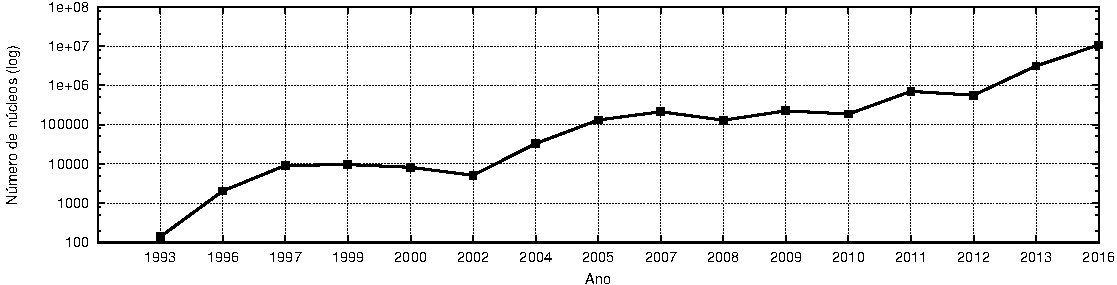
\includegraphics[width=\textwidth]{figs/top500.pdf} \\
    Fonte: desenvolvido pelo autor.
	\label{fig:graphCores}
\end{figure}

% \todo[inline]{Saiu a lista de novembro. Atualizar o gráfico e o texto.}

\begin{figure}[t]
	\centering
	\caption{Eficiência energética do supercomputador número 1 do
        \textit{ranking} Green500 (dados extraídos do site Green500).}
    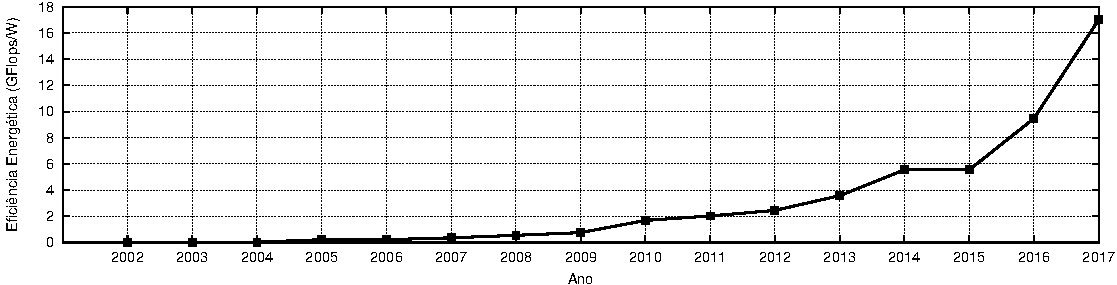
\includegraphics[width=\textwidth]{figs/green500.pdf} \\
    Fonte: desenvolvido pelo autor.
	\label{fig:graphEnergy}
\end{figure}


Até a última década, o desempenho das arquiteturas utilizadas em \hpc era quantificado quase
que exclusivamente pelo seu poder de processamento, usualmente medido por
\flops. Contudo, o consumo excessivo de energia é uma barreira para o aumento de
desempenho de forma escalável nestas plataformas.
Essa preocupação com o aumento de energia é ressaltada pelo relatório emitido
pelo Departamento de Defesa do Governo dos Estados Unidos (DARPA/IPTO)
~\cite{Kogge2008}. O relatório ressalta que a potência máxima aceitável para supercomputadores
\textit{Exascale} (10$^{18}$ \flops) seria de 20 MW\footnote{Atualmente, a
    potência máxima está sendo considerada em até 30 MW}, isto é, com
essas características, um supercomputador deveria possuir uma eficiência
energética de 50 GFlops.
Por outro lado, atualmente, os supercomputadores mais energicamente eficientes
possuem uma eficiência energética de no máximo $17$ GFlops/W, como pode ser observado nos dados extraídos do \textit{ranking}
Green500\footnote{\url{https://www.top500.org/green500/}} mostrados na Figura~\ref{fig:graphEnergy}.
Este valor é quase 3 vezes menor que o ressaltado pelo
relatório da DARPA/IPTO, sendo assim, atualmente a eficiência energética de
supercomputadores está ainda distante da ideal. Portanto, para que
supercomputadores tenham potencial para atingir o \textit{Exascale} é necessário
um consumo energético viável e um alto desempenho. Contudo, o crescimento dessas
duas variáveis não é proporcional.


Por essa razão, o estudo de técnicas que melhorem a eficiência energética em
plataformas \hpc está se tornando muito importante.  Recentemente, uma nova
classe de processadores \textit{manycore} de baixa potência, tais como, o Sunway
SW26010~\cite{sunway:2016}, Mellanox TILE-Gx~\cite{Valero:2012} e Kalray
\mppa~\cite{Castro-IA3:2013}, foi desenvolvida. Esses processadores possuem
centenas de núcleos de processamento capazes de lidar com paralelismo de dados e
tarefas com baixo consumo de energia.

Apesar desses processadores \textit{manycore} fornecerem uma melhor eficiência
energética~\cite{Castro-IA3-JPDC:2014}, eles possuem uma arquitetura particular
que torna o desenvolvimento de aplicações paralelas uma tarefa
desafiadora~\cite{Varghese14,Castro-PARCO:2016,Castro-SBAC-PAD:2014}. Núcleos de
processamento sem coerência de \textit{cache} são, geralmente, distribuídos em
uma arquitetura organizada em \textit{clusters}, onde cada \textit{cluster}
possui uma memória local (compartilhada somente entre os núcleos do
\textit{cluster}). Dessa forma, a comunicação entre \textit{clusters} deve ser efetuada através de uma \noc de maneira distribuída.
Por essa razão, o tempo de comunicação pode variar entre os núcleos que estão se
comunicando.
%Explicar as dificuldades.

O \mppa possui 256 núcleos distribuídos em 16 \textit{clusters}, denominados
\pes, e 4 subsistemas de \es. O ambiente do \mppa é heterogêneo, sendo
utilizada, entre os \textit{clusters} e subsistemas, uma comunicação via \noc e
dentro de cada \textit{cluster} são utilizadas comunicações diretas entre
\pes, por meio de memória compartilhada. As principais dificuldades do
desenvolvimento de aplicações para o \mppa são resumidas a seguir:

\begin{itemize}
	\item \textbf{Modelo de programação híbrido}: problema citado anteriormente, onde \textit{threads}
em um mesmo \textit{cluster} se comunicam através de memória compartilhada
local, porém a comunicação entre \textit{clusters} é feita explicitamente via
NoC, seguindo um modelo de computação distribuída;
	\item \textbf{Comunicação explícita}: é necessária a utilização de uma \api
específica para a comunicação via NoC, similar ao \posix de baixo nível para
\ipc;
	\item \textbf{Memória limitada}: cada \textit{cluster} possui apenas 2MB de memória
local de baixa latência, portanto aplicações reais precisam constantemente
realizar comunicações com o subsistema de \es;
	\item \textbf{Ausência de coerência de \textit{cache}}: cada PE possui uma memória \textit{cache} privada e sem coerência
com as \textit{caches} dos demais PEs, sendo necessário atualizar a \textit{cache} manualmente.
\end{itemize}

Uma possível solução para os problemas apresentados anteriormente é a utilização de padrões
paralelos ou esqueletos~\cite{cole-skeleton:2004}. Esqueletos
são modelos de programação paralela de alto nível de abstração. Esses modelos fornecem
vantagens para o desenvolvedor, escondendo a complexidade de aplicações
paralelas e distribuídas. Os esqueletos especificam, mais precisamente,
os padrões de acesso de dados e comunicação. Desta forma, eles possibilitam aos
desenvolvedores focarem apenas nos algoritmos, ao invés da comunicação,
sincronização de tarefas e escalonamento, que são gerenciados de forma
transparente pelo \fw que implementa um esqueleto.
Entre os diversos esqueletos existentes (\textit{map}, \textit{reduce},
\textit{pipeline} e \textit{scan}), o padrão \stencil é
utilizado em ambientes industriais e acadêmicos, como física quântica, previsão do tempo e
processamento de imagens~\cite{gonzalez06,holewinski12}.

%Explicar Stencil? Imagens?

\Fws são utilizados para fornecer uma abstração sobre partes de código que serão
reusadas diversas vezes. Esse \fw pode ser estendido ou adaptado para fornecer
suporte para outras aplicações com diferentes características. Dessa forma, a
utilização de um \fw pode facilitar o desenvolvimento de aplicações para
ambientes onerosos, como ambientes \textit{manycore}.

Muitos \fws foram propostos para o auxílio no desenvolvimento de aplicações paralelas do
padrão estêncil, como o
PSkel~\cite{pereira15}, SkePU~\cite{enmyren10} e SkelCL~\cite{steuwer11}. Em
particular, o PSkel é um \fw que fornece uma abstração em alto nível para o
desenvolvimento em ambientes heterogêneos CPU-GPU, enquanto particiona tarefas e
dados de forma transparente entre esses processadores.
%\section{Motivação}

\section{Objetivos}

Com base no exposto, são apresentados a seguir o objetivo geral e os objetivos específicos
do presente projeto.

\subsection{Objetivo Geral}

O objetivo principal deste TCC é propor uma adaptação do \fw \pskel para o processador \textit{manycore}
emergente denominado \mppa, facilitando assim o desenvolvimento de aplicações \stencil neste processador.
A adaptação permitirá que aplicações já existentes do \pskel possam ser executadas
no \mppa sem nenhuma necessidade de alteração de código.

\subsection{Objetivos Específicos}

\begin{itemize}
	\item Definir uma estratégia de distribuição de dados entre os \textit{clusters} do \mppa a fim de
	lidar com a capacidade limitada de memória no \textit{chip};
	\item Propor e implementar técnicas que permitam reduzir os custos de comunicação na \noc;
	\item Adaptar as principais classes e abstrações existentes no \pskel para o processador \mppa;
	\item Realizar uma análise do desempenho e do consumo de energia da solução proposta para o \mppa
	utilizando diversas aplicações estêncil já implementadas no \pskel;
	\item Realizar comparações de desempenho e consumo de energia com um processador \textit{multicore} atual.
\end{itemize}

\section{Contribuições do Trabalho}

As contribuições principais deste trabalho foram publicadas em diferentes eventos da área de Computação Paralela e Distribuída.
Abaixo são apresentados os artigos publicados:

\begin{itemize}
    \item PODESTA JUNIOR, E. ; MARQUES, B. ; CASTRO, M. \textbf{Energy Efficient
            Stencil Computations on the Low-Power Manycore MPPA-256 Processor}.
        In: Conferência Européia Internacional de Computação Paralela e
        Distribuída (EURO-PAR), 2018, Turin, Itália.

	\item PODESTA JUNIOR, E. ; PEREIRA, A. D. ; ROCHA, R. C. O. ; CASTRO, MÁRCIO ; GOES, L. F. W. \textbf{Execução Energeticamente Eficiente de Aplicações Estêncil com o Processador Manycore MPPA-256}. In: Simpósio em Sistemas Computacionais de Alto Desempenho (WSCAD), 2017, Campinas. Anais do Simpósio em Sistemas Computacionais de Alto Desempenho (WSCAD). Porto Alegre: SBC, 2017. v. 1. p. 52-63.

	\item PODESTA JUNIOR, E. ; PEREIRA, A. D. ; ROCHA, R. C. O. ; CASTRO, M. ; GOES, L. F. W. \textbf{Uma Implementação do Framework PSkel com Suporte a Aplicações Estêncil Iterativas para o Processador MPPA-256}. In: Escola Regional de Alto Desempenho do Estado do Rio Grande do Sul (ERAD/RS), 2017, Ijuí. Anais da Escola Regional de Alto Desempenho do Estado do Rio Grande do Sul (ERAD/RS). Porto Alegre: Sociedade Brasileira de Computação, 2017. v. 1. p. 395-398.

	\item PODESTA JUNIOR, E. ; PEREIRA, A. D. ; PENNA, P. H. ; ROCHA, R. C. O. ; CASTRO, M. ; GOES, L. F. W. \textbf{PSkel-MPPA: Uma Adaptação do Framework PSkel para o Processador Manycore MPPA-256}. In: Escola Regional de Alto Desempenho do Estado do Rio Grande do Sul (ERAD/RS), 2016, São Leopoldo. Anais da Escola Regional de Alto Desempenho do Estado do Rio Grande do Sul (ERAD/RS). Porto Alegre: Sociedade Brasileira de Computação (SBC), 2016.
\end{itemize}

\section{Organização do Texto}
O texto deste trabalho será organizado da seguinte forma. O Capítulo~\ref{cha:fundTeorica} descreve a base conceitual
utilizada para realizar este trabalho. O Capítulo~\ref{cha:trabalhos-relacionados} discute os principais trabalhos relacionados.
O Capítulo~\ref{cha:proposta} apresenta a proposta de adaptação do \pskel para o \mppa.
O Capítulo~\ref{cha:experimentos} apresenta a análise experimental dos resultados. Por fim, o
Capítulo~\ref{cha:conclusao} conclui este trabalho.
% Introduzir Figura
%\begin{figure}
%	   \centering
%	   		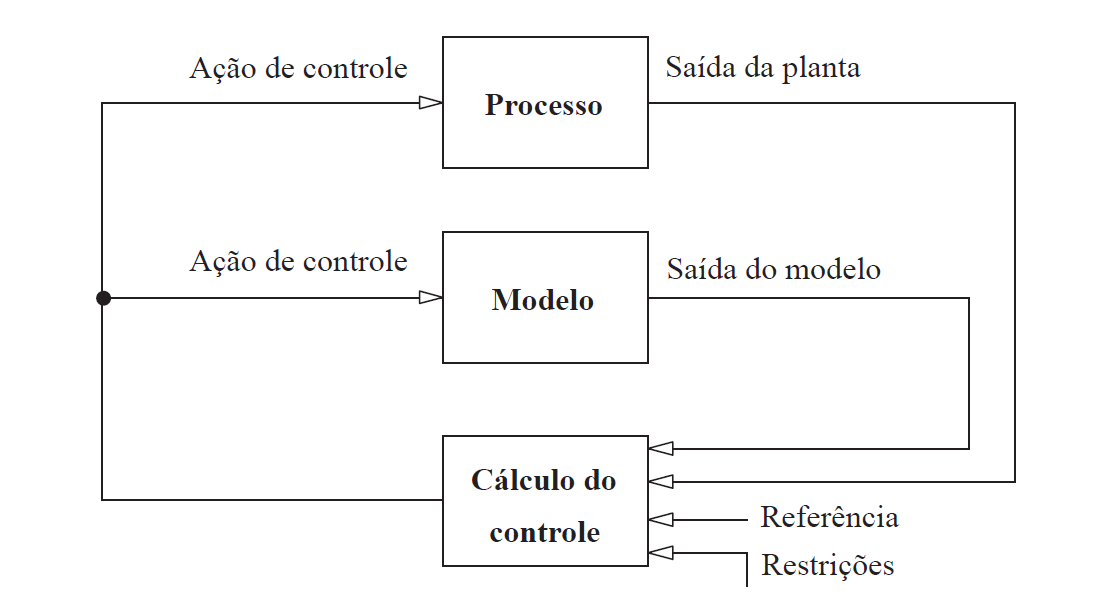
\includegraphics[scale=0.35]{figs/MPCbase.PNG}
%	   \caption{Algoritmo MPC}
%	   \label{label para referencia cruzada Figura}
%\end{figure}


% Lista de Item

%\begin{itemize}
%	\item item 1
%	\item item 2
%	\item item 3
%\end{itemize}

% Equação
%\begin{equation}
%	\label{label para referencia cruzada %equacoes}
%	y(t)=\sum_{i=1}^{\infty}h_i\Delta u(t-i)
%\end{equation}

% Equação em linha
%$\hat{y}(t+k\mid t)= \sum^\infty_{i=1} g_i %\Delta u(t+k-i\mid t)$

% Citação -  Criei o arquivo de bibliografia usando o jabref

%\cite{Camacho2007}

% Referencia Cruzada de Figura
%\ref{label para referencia cruzada Figura}

% Referencia Cruzada de Equação
%\ref{label para referencia cruzada equacoes}


% Tabelas

%\begin{table}[h]
%\begin{center}
%     \caption{Índices 1 para casos factíveis}
%     \begin{tabular}{| l | l | l | l |}
%     \hline Índice & LP Petro & LP 2 & %Diferença\\
%     \hline $SES_y$& 60.5406 & 60.5492 & %-0.0087\\
%     \hline $SES_u$& 1166.1464 & 1166.1464 & 2.36*$10^{-9}$ \\
%     \hline

%    \end{tabular}
%\label{table:indices1}
%\end{center}
%\end{table}

\chapter{Fundamentação Teórica}
\label{cha:fundTeorica}

Esta seção apresenta uma fundamentação teórica básica sobre Computação Paralela sob
o ponto de vista arquitetural (Seção~\ref{sec:arquiteturas}) e de programação (Seção~\ref{sec:prog-paralela}).
Posteriormente, serão apresentados os conceitos fundamentais do padrão \stencil (Seção~\ref{sec:stencil}) e
sobre o \fw \pskel (Seção~\ref{sec:pskel}).

\section{Arquiteturas Paralelas}
\label{sec:arquiteturas}

De acordo com Tanenbaum~\etal~\cite{Tanenbaum2015}, as arquiteturas paralelas podem ser classificadas em
dois grandes grupos: multiprocessadores e multicomputadores. Nas seções a seguir são apresentados os
principais conceitos básicos destas duas classes de arquiteturas paralelas. Posteriormente, será discutido
em mais detalhes o processador \textit{manycore} \mppa, o qual será utilizado neste trabalho.

% \todo[inline]{Para o restante desta seção, tu podes pegar informações do livro do Tanenbaum de SO. O capítulo 8
% trata sobre multiprocessadores (seção 8.1) e multicomputadores (seção 8.2)}

\subsection{Multiprocessadores}

% \todo[inline]{
% - Organização: processadores interconectados a uma memória compartilhada via barramento (UMA). Podes usar a figura
% 8.2c do livro como base para fazer uma tua e mostrar as ideias.
% }

% \todo[inline]{
% - Podes falar rapidamente sobre NUMA e as diferenças para o UMA.
% }

% \todo[inline]{
% - Então, podes entrar no assunto dos multicores:

Multiprocessadores são sistemas constituídos de uma ou mais \cpus que
compartilham totalmente
a \ram do sistema. Desta forma, \textit{threads} de um mesmo processo se
comunicam através do mesmo espaço de endereçamento, por meio de escrita e
leitura na memória. Essa característica do sistema pode ocasionar problemas de
concorrência, onde um valor escrito por uma \textit{thread}, localizado em uma
palavra na memória, pode ser alterado por outra \textit{thread}, trazendo
inconsistência ao sistema.

Mais especificamente, multiprocessadores podem possuir propriedades adicionais,
como acesso uniforme à memória. Máquinas com essa propriedade são chamadas de
\uma. Por outro lado, existem multiprocessadores que não apresentam essa
característica, como é o caso de multiprocessadores \numa, que apresentam um acesso
não-uniforme à memória.

%\todo[inline]{\uma e \numa aparecem aqui pela primeira vez mas o nome não ficou por extenso.
%verificar o que está acontecendo...}

A Figura~\ref{fig:uma} apresenta a arquitetura de sistemas multiprocessados \uma
mais simplificados, onde existem várias \cpus que se
comunicam com uma memória compartilhada por meio de um barramento. Quando uma
\cpu deseja efetuar a comunicação, o barramento é verificado para
determinar a sua disponibilidade. Caso o barramento esteja ocupado, a
\cpu espera até que ele fique livre. Com o barramento livre, a \cpu
coloca o endereço da palavra no barramento, utiliza sinais de
controle e espera até que a memória coloque a palavra desejada no barramento. Esse
método é gerenciável para poucas \cpus, contudo com uma maior quantidade, o
número de comunicações aumenta significativamente, tornando
o gerenciamento de comunicações, por meio do barramento, insuportável. Desta
forma, o barramento se torna o gargalo do sistema.

\begin{figure}[t]
	\centering
    \caption{Esquema genérico de um multiprocessador \uma.}
    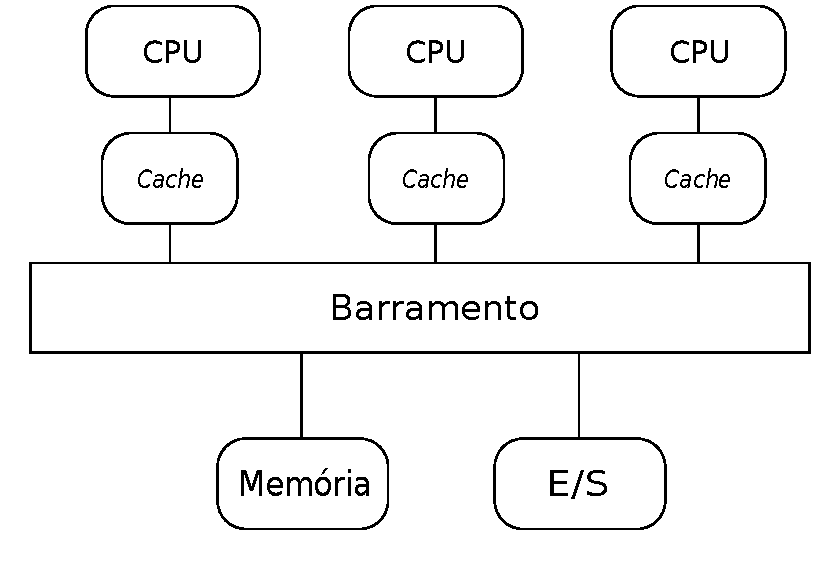
\includegraphics[width=0.5\textwidth]{figs/multiproc.pdf} \\
    Fonte: desenvolvido pelo autor.
    \label{fig:uma}
\end{figure}

A solução é utilizar \textit{caches} nas \cpus, possibilitando que requisições
de leitura sejam satisfeitas pela \textit{cache}, diminuindo a quantidade de
comunicações. Desta forma, é possível adicionar mais \cpus no barramento devido à baixa
quantidade de tráfego. \textit{Caches} possuem protocolos de coerência para
manter a consistência do sistema. Quando uma \cpu
efetua uma escrita sobre uma palavra, todas as \textit{caches} que possuem essa
palavra serão notificadas. Uma \textit{cache} com uma cópia modificada, isto é,
diferente do dado presente na memória, deve escrever essa cópia diretamente na
memória. Caso uma cópia exata do dado na memória esteja presente na
\textit{cache}, ela pode ser descartada, fazendo com que a \cpu acesse
diretamente a memória.

Além disso, é possível inserir mais níveis de \textit{cache} nas \cpus,
diminuindo o tráfego e retirando a necessidade de mais acessos à memória
principal. Contudo, devido ao limite arquitetural, uma quantidade muito grande
de \textit{caches} é inviável. Além disso, um tamanho muito grande para
\textit{caches} torna o seu acesso muito lento, prejudicando o desempenho do
sistema.

Sistemas multiprocessados \numa são diferentes de sistemas \uma, como mencionado
anteriormente, devido ao acesso à memória remota ser mais lento que à memória
local. A Figura~\ref{fig:numa} apresenta a arquitetura desse sistema, onde
existem nós interconectados por uma rede, e cada nó possui uma \cpu e um bloco
de memória. A \cpu de cada nó pode possuir uma \textit{cache}, denominada
\ccnuma, que possibilita uma redução no tempo de acesso a um dado localizado em
uma memória remota. Por outro lado, um sistema sem \textit{cache} é
denominado \ncnuma.

\begin{figure}[t]
	\centering
    \caption{Esquema genérico de um multiprocessador \numa.}
    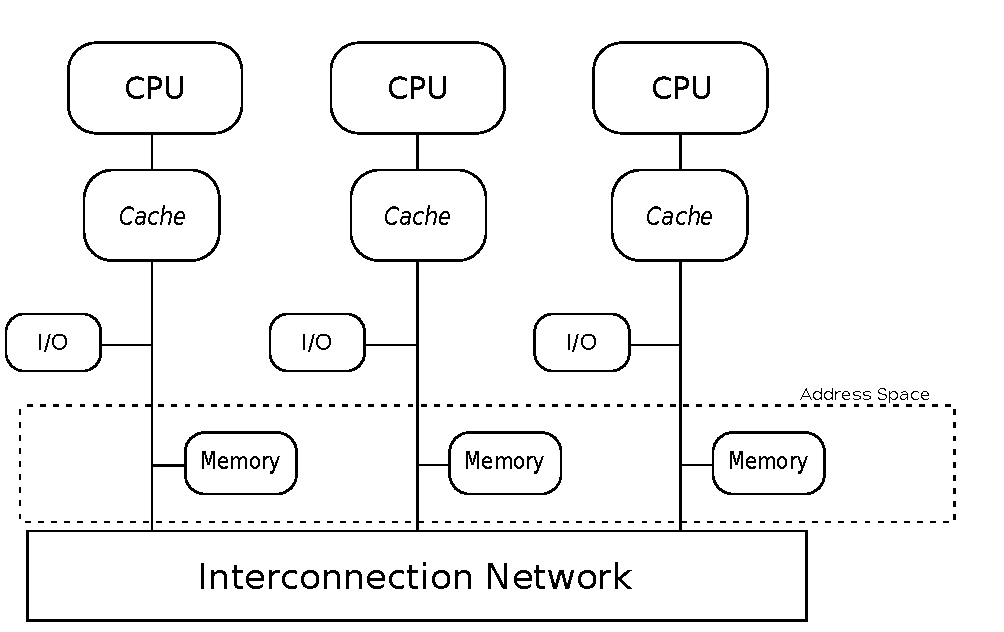
\includegraphics[width=0.6\textwidth]{figs/multiprocNUMA.pdf} \\
    Fonte: desenvolvido pelo autor.
    \label{fig:numa}
\end{figure}

Com o desenvolvimento de novas tecnologias, o tamanho
dos transistores diminuiu significativamente, se tornando possível inserir um
grande número de transistores em um único \textit{chip}.
Com o aumento da quantidade de transistores, um \textit{chip} pode ter, por
exemplo, várias \cpus, denominadas \textit{cores}, caracterizando um
\textit{chip} \textit{multicore}.
Geralmente chamados de \cmps, os \textit{multicores} são semelhantes aos multiprocessadores
tradicionais, contudo, devido à proximidade de conexão entre \cpus, falhas em um
componente pode ocasionar problemas em outros componentes do sistema.
Esse problema pode ser ainda mais agravado em sistemas do tipo \mpsoc. Esses sistemas
possuem geralmente \cpus (muitas vezes \textit{multicore}) de propósito geral, além de processadores
dedicados a atividades bem específicas, tais como decodificadores de áudio e vídeo, processadores
criptográficos, entre outros. Além dos processadores, esses sistemas também incluem diferentes tipos
de interface de rede e de \es no mesmo \textit{chip}.

Quando a quantidade de \textit{cores} é grande, isto é, dezenas ou milhares de
\textit{cores}, o \textit{chip} pode ser classificado como \textit{manycore}.
Contudo, o limite para classificar um \textit{chip} em \textit{manycore} ou
\textit{multicore} é flexível~\cite{Tanenbaum2015}.
Atualmente, aceleradores com uma grande quantidade \textit{cores} estão
surgindo, como o Xeon Phi da Intel com 60 \textit{cores}.

Com vários \textit{cores} em um único \textit{chip} problemas de coerência de
\textit{cache} começam a surgir. Mais especificamente, com o aumento no número
de \textit{cores}, o custo sobre o protocolo de coerência vai crescer até que
aumentar o número de \textit{cores} não auxiliará mais o desempenho, pois o sistema
estará gastando muito tempo mantendo as \textit{caches} consistentes.


Atualmente, sistemas computacionais comuns apresentam uma \gpu, onde temos
milhares de \textit{cores} disponíveis. \gpus utilizam esses \textit{cores},
essencialmente, para a solução de cálculos, focando menos em questões de
\textit{cache} e lógica de controle. Desta forma, elas são utilizadas em
pequenas computações que podem ser paralelizadas. Contudo, a programação para
\gpus é difícil, pois os seus \textit{cores} fazem a execução da mesma instrução
com diferentes partes do dado, isto é, são máquinas \simd. Esse modelo de
programação é interessante para abordar o paralelismo de dados, contudo, o
desenvolvedor pode se deparar com dificuldades durante o desenvolvimento.
Desta forma, linguagens de programação, como CUDA e \opencl,
abstraem o desenvolvimento de aplicações para esses processadores.

O \mppa é um processador \textit{manycore} diferente dos apresentados acima,
pois os seus \textit{cores} são conectados atraves de uma \noc. Mais detalhes
sobre o \mppa serão apresentados posteriormente na Seção~\ref{sec:mppa}, tendo
em vista que ele possui também características relacionadas a multicomputadores.

% Até a última década, o desempenho sobre computadores escalava de acordo com o
% aumento da frequência dos processadores.
%
%
% Contudo, com o aumento da frequência,
% a potência e o consumo de energia também aumentam. De acordo com a
% Equação~\eqref{eq:power}, pode-se perceber que a potência aumenta,
% proporcionalmente, com o aumento da frequência.
%
%
% \begin{equation}\label{eq:power}
% 	P = CV^2f
% \end{equation}
%
% \todo[inline]{Esta parte está ruim. 1) Não foi explicada a equação (o que é P, C, V e f?).
% 2) Dizer que a potência aumenta proporcionalmente com o aumento da frequência não está totalmente correto,
% pois a tensão (V) também tem relação com a frequência (f). A tensão tem um impacto ainda maior, pois
% ela é quadrática na equação. Tens que dar uma olhada melhor nisso e corrigir o texto.}
%
% Portanto, o aumento do desempenho encontrou uma barreira no consumo de energia, onde tornou-se inviável
% um aumento indiscriminado da frequência. Desta forma, tornou-se necessário uma
% nova abordagem para aumentar o desempenho dos processadores. A solução encontrada
% pelos fabricantes de \textit{chips} foi de aumentar a quantidade de núcleos processamento no \textit{chip},
% porém reduzindo a frequência de operação dos mesmos, dando origem aos processadores \textit{multicore}.
%
% \todo[inline]{
% - Falar de \textit{manycores} (de modo geral), dando exemplos: Xeon Phi e GPU, que são dois tipos de \textit{manycores}
% bem diferentes.
% }
%
% \todo[inline]{
% - Finalizar dizendo que o \textit{manycore} utilizado neste trabalho se diferencia dos dois exemplos anteriores, pois
% seus núcleos são conectados através de uma NoC. Então, diz que será tratado desse assunto na Seção 2.1.3
% }
%
\subsection{Multicomputadores}

% \todo[inline]{
% - Organização: sistemas multiprocessados, cada um com sua memória de dedicada, conectados através de uma rede. Podes usar
% a figura 8-18 como base para explicar as ideias.
% }
%
% \todo[inline]{
% - Podes falar rapidamente dos diferentes tipos de interconexão: figura 8-16 do livro
% }
%
% \todo[inline]{
% - Falar dos tipos de multicomputadores: NOW, COW, etc...
% }
%
% \todo[inline]{
% - Finalizar indicando que nos multicomputadores a comunicação entre os processadores é feita de maneira explícita através de trocas de mensagens.
% }
%
Multiprocessadores de grande porte são difíceis de construir devido ao alto
custo. Desta forma, devido à simplicidade de construção, multicomputadores
começaram a surgir. A ideia principal de um multicomputador é agregar em um mesmo sistema diversos
computadores, os quais muitas vezes possuem multiprocessadores~\cite{Tanenbaum2015}.
Nesse sentido, um computador com sua placa de interface de rede é considerado como um nó do
sistema multicomputado, onde um gerenciamento de forma inteligente da rede auxilia o desempenho
do sistema.

\begin{figure}[t]
	\centering
    \caption{Esquema simples de um sistema multicomputado.}
        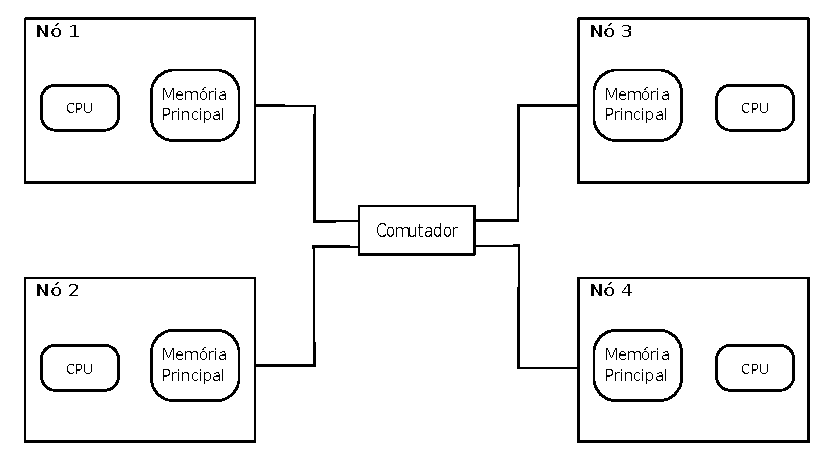
\includegraphics[width=0.7\textwidth]{figs/multicomp.pdf} \\
        Fonte: desenvolvido pelo autor.
        \label{fig:multicomputado}
\end{figure}



A Figura~\ref{fig:multicomputado} mostra como um sistema multicomputado simples é
organizado. Existem nós que possuem uma \cpu, memória principal dedicada e uma
conexão diretamente com outros nós ou a um comutador. A topologia apresentada na
imagem é uma das topologias possíveis em um sistema multicomputado. Outra
alternativa é utilizar uma topologia em anel (Figura~\ref{fig:topologia}b), retirando a necessidade de um
comutador, pois um nó é conectado diretamente aos outros nós. Cada nó é
conectado ao nó à sua esquerda e à sua direita.

Uma outra topologia de interconexão muito utilizada em multicomputadores é a malha (\textit{mesh}),
a qual é ilustrada pela Figura~\ref{fig:topologia}c. Nesse tipo de topologia, os nós são interconectados
em comutadores distintos pelo sistema e cada comutador é conectado a outros
comutadores, formando uma espécie de malha no sistema. Uma variante dessa
topologia é o toro duplo (\textit{torus}) apresentado na Figura~\ref{fig:topologia}d, onde os
comutadores de cantos opostos estão conectados diretamente. Desta forma,
comunicações entre nós de cantos opostos não terão a necessidade de inúmeros
saltos pelos comutadores para efetuar a transmissão de informações.

A Figura~\ref{fig:topologia}e ilustra uma topologia tridimensional, e a
Figura~\ref{fig:topologia}f ilustra um cubo tetradimensional. Topologias
$n$ dimensionais são utilizadas para diminuir o atraso de comunicação entre nós,
pois o diâmetro da rede cresce linearmente de acordo com a dimensionalidade.
Devido a essa propriedade, topologias $n$ dimensionais são utilizadas em
vários sistemas.

\begin{figure}[t]
	\centering
        \caption{Topologias de interconexão.}
	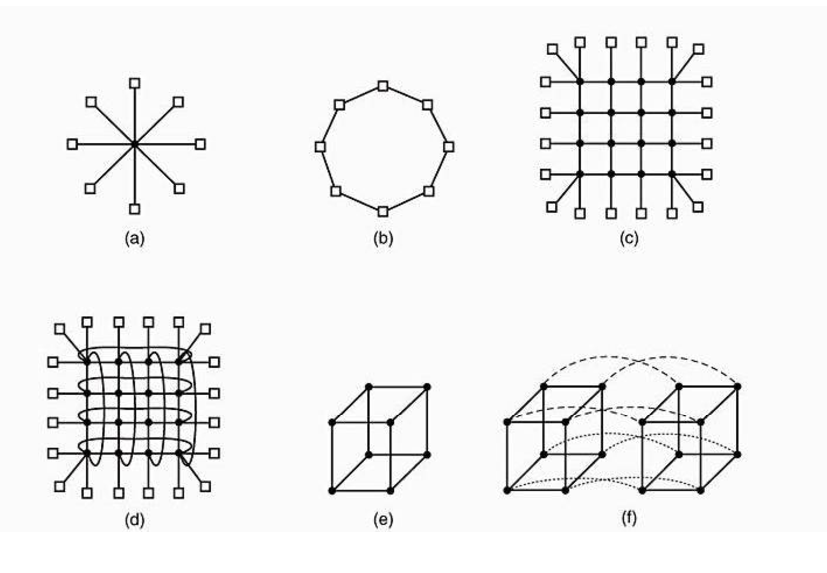
\includegraphics[width=\textwidth]{figs/topologia.pdf} \\
    Fonte:~\cite{Tanenbaum2015}
    \label{fig:topologia}
\end{figure}


%Cow Now
Geralmente, multicomputadores podem ser construídos com computadores pessoais
comuns interconectados por uma \textit{interface} de rede para trabalharem em
conjunto. Organizações de multicomputadores deste tipo são denominadas de \now. Devido à sua
simplicidade, esse sistema não é focado em ganho de desempenho. Por outro lado, \cow
são constituídos de computadores interconectados sem teclado, monitor e \textit{mouse} contendo cada
um diversos processadores de alto desempenho. Esses sistemas são focados em desempenho, pois
possuem redes de interconexão de alto desempenho (alta largura de banda e baixa latência).

A comunicação em um multicomputador é feita por meio de troca de mensagens.
Processos localizados em diferentes \cpus se comunicam por meio de mecanismos básicos
disponibilizados pelo \so. Esses mecanismos básicos do \so são utilizados como base para implementação
de bibliotecas de comunicação que implementam, pelo menos, duas primitivas básicas: \textit{send} e \textit{receive}.
A primitiva \textit{send} envia uma mensagem para um processo, o que é determinado pelos
parâmetros de entrada da mesma. A primitiva \textit{receive} é responsável pelo recebimento
de mensagens, utilizando como parâmetro o endereço que será lido para coletar a
mensagem recebida. Portanto, em sistemas multicomputados a troca de mensagens
entre processos é realizada de maneira explícita pelo desenvolvedor.


\subsection{O Processador \textit{Manycore} MPPA-256}
\label{sec:mppa}

O \mppa é um processador \textit{manycore} desenvolvido pela empresa francesa
Kalray, o qual possui 256 núcleos de processamento de 400 MHz. Ele mistura características
de um multiprocessador e de um multicomputador, porém em um único \textit{chip}.
Mais especificamente, o \mppa utiliza um modelo multicomputado com uma
comunicação via \noc em seus \textit{clusters}, e um modelo multiprocessado
dentro de cada \textit{cluster}.

\begin{figure}[t]
	\centering
	\caption{Visão geral do \mppa.}
	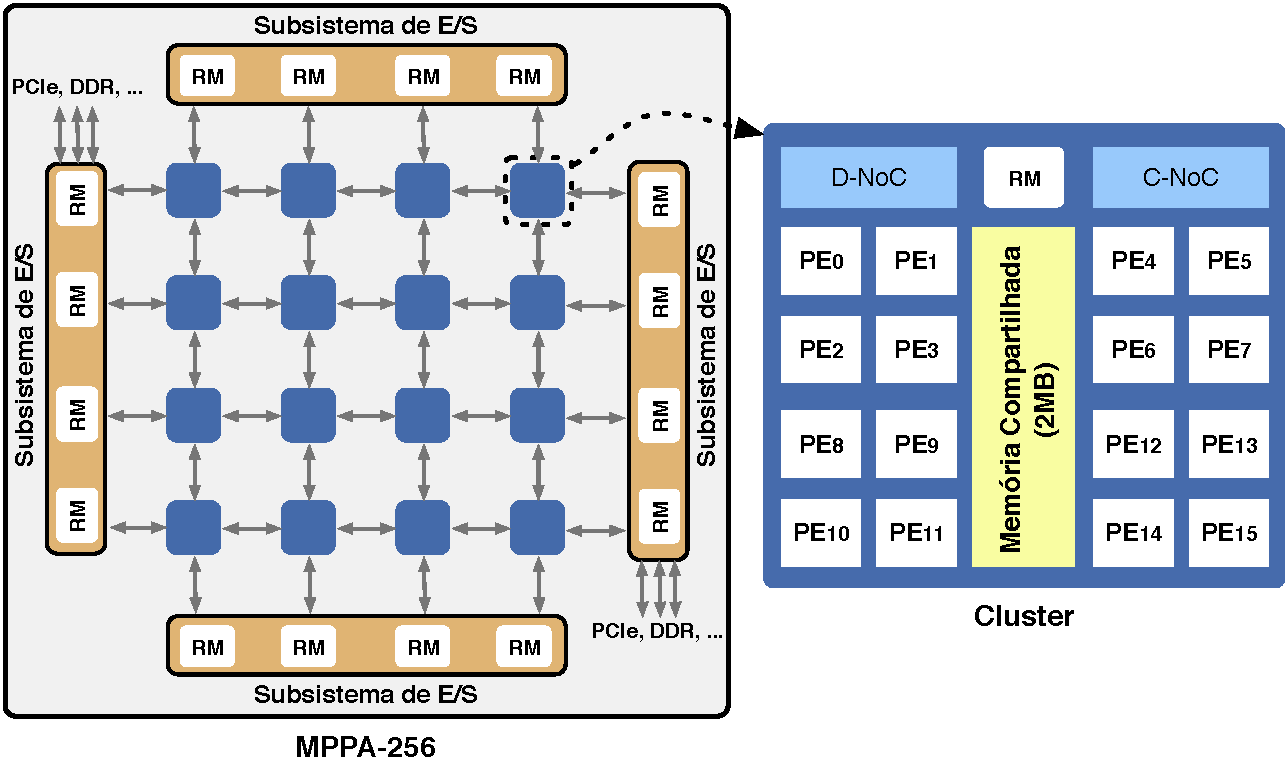
\includegraphics[width=0.9\textwidth]{figs/mppa-overall.pdf} \\
    Fonte:~\cite{Castro-IA3:2013}
	\label{fig:mppa}
\end{figure}

Os núcleos de processamento do \mppa são denominados \pes.
Além dos \pes, o processador possui 32 núcleos dedicados à gerência de recursos
denominados  \rmans. \pes e \rmans são distribuídos
fisicamente no \textit{chip} em 16 \textit{clusters} e 4 subsistemas de \es,
contendo cada \textit{cluster}, 16 \pes e 1 \rman. Além dos \textit{clusters}, o
\mppa possui 4 subsistemas de \es contendo, cada um, 4 \rmans. Toda a comunicação
entre \textit{clusters} e/ou subsistemas de \es é feita através de uma \noc
\textit{torus} 2D. A arquitetura do \mppa pode ser vista na
Figura~\ref{fig:mppa}\footnote{A figura apresenta uma ilustração simplificada,
    omitindo a topologia da \noc.}.

A finalidade principal dos \pes é executar \textit{threads} de usuário de forma
ininterrupta e não preemptível para realização de computação. \pes de um mesmo
\textit{cluster} compartilham uma memória de 2~\mb, a qual é utilizada para
armazenar os dados a serem processados pelos \pes. Cada \pe possui também uma
memória \textit{cache} associativa 2-\textit{way} de 32~\kb para dados e uma para
instruções. Porém, o processador não dispõe de coerência de \textit{caches}, o
que dificulta o desenvolvimento de aplicações para esse processador. Por outro
lado, a finalidade dos \rmans é gerenciar \es, controlar comunicações entre
\textit{clusters} e/ou subsistemas de \es e realizar comunicação com uma memória
\ram. Na arquitetura utilizada neste trabalho, um dos subsistemas de \es está conectado a uma
memória externa \lpddr de 2~\gb.

A comunicação dos \textit{clusters} com o subsistema de \es e a comunicação
entre \textit{clusters} é realizada de maneira explícita, utilizando uma \api
própria do \mppa de baixo nível similar à \posix \ipc. Detalhes referentes à
comunicação e programação nesse processador serão abordadas posteriormente
na Seção~\ref{sec:prog-mppa}.

% - Terminar essa seção falando que a comunicação entre clusters e entre cluster/IO tem
% que ser feita de maneira explícita utilizando uma API de baixo nível. Então, diz que os detalhes
% referentes a programação nesse processador serão tratados na Seção 2.2.3
%----------------------------------------------------------------------------------------
%Existem diversos tipos de arquiteturas que proporcionam ao desenvolvedor uma
%abordagem paralela. Multiprocessadores são arquiteturas que fornecem vários
%núcleos de processamento em uma máquina e a comunicação entre os núcleos é feita
%através da memória compartilhada, contudo este modelo traz dificuldades em
%relação à organização e particionamento de dados entre núcleos. Devido ao espaço
%limitado em \textit{chip}, o aumento do número de núcleos nessa arquitetura pode
%se tornar inviável, portanto, arquiteturas multicomputadas são utilizadas, onde
%temos várias máquinas, sendo, geralmente, multiprocessadas, interligadas para
%fornecer um maior poder de processamento. A comunicação entre cada
%\textit{cluster}, isto é, cada nó na rede de computadores utiliza distribuição
%de dados e sincronizações, como não temos compartilhamento de memória entre os
%nós de processamento, o desenvolvimento de código para essa arquitetura é mais
%complicada, pois existem vários fatores à serem avaliados pelo desenvolvedor. Na
%próxima seção serão abordadas as dificuldades e implementação de cada modelo.

%Arquiteturas paralelas: multicomputadores, multiprocessadores, compartilhamento de memória e distribuição de dados.
%Programação paralela: uso de apis, dificuldades. POSIX, MPI...


\section{Programação Paralela}
\label{sec:prog-paralela}

Aplicações são, geralmente, implementadas de forma
sequencial, isto é, um conjunto serializado de instruções que será executado
sobre uma \cpu. Por outro lado, a computação paralela ou distribuída efetua o
processamento de instruções sobre múltiplos elementos de processamento. A ideia
principal é dividir a computação em partes menores que podem ser executadas
simultaneamente entre os elementos de processamento distintos, com intuito de se
realizar um processamento em menos tempo.

Diferentes \apis de programação paralela foram criadas com intuito de simplificar
o desenvolvimento de aplicações em arquiteturas multiprocessadas e multicomputadas.
A seguir serão apresentadas as \apis mais utilizadas no âmbito de \hpc em cada tipo de
arquitetura. Por fim, será apresentada a \api utilizada para o desenvolvimento de aplicações
no processador \mppa.


\subsection{OpenMP}

% \todo[inline]{
% - Dizer que é feita para ser utilizada em arquiteturas multiprocessadas, ou seja, com memória
% compartilhada.
% }
%
% \todo[inline]{
% - Apresentar as principais ideias do OpenMP: dizer que é baseada em pragmas, modelo fork-join,
% regiões paralelas, paralelização de laços, ... (A \api é baseada no modelo de programação
% paralela de memória compartilhada, apresentando uma boa portabilidade e pouco
% esforço de programação. O modelo de programação utiliza diretivas de compilação
% e variáveis, tornando possível poucas modificações de código para utilizar
% outras \textit{threads} na aplicação....)
% }


Para evitar uma programação de baixo nível sobre um sistema multiprocessado, são
utilizadas \apis para o desenvolvimento de aplicações, como o OpenMP. O OpenMP
é um modelo de programação baseado em memória compartilhada, e apresenta boa
portabilidade, um bom desempenho e escalabilidade. Devido à abstração que a \api
fornece, o desenvolvimento de aplicações para o ambiente multiprocessado é
facilitado, permitindo paralelização de aplicações com variáveis de ambiente e
diretivas de compilação.

O OpenMP utiliza o modelo \textit{fork-join}, onde a execução inicia com uma
única \textit{thread}, denominada \textit{master thread}. Como ilustrado na
Figura~\ref{fig:forkjoin}, quando a \textit{master thread} encontra
uma região paralela, são criadas outras \textit{threads} de acordo com a variável
de ambiente especificada no sistema. No final da região paralela, é realizado um
\textit{join} por meio de uma barreira implícita, onde as \textit{threads} serão
sincronizadas, e a execução irá continuar apenas com a \textit{master thread}.

\begin{figure}[t]
	\centering
	\caption{Esquemático do modelo \textit{fork-join}.}
	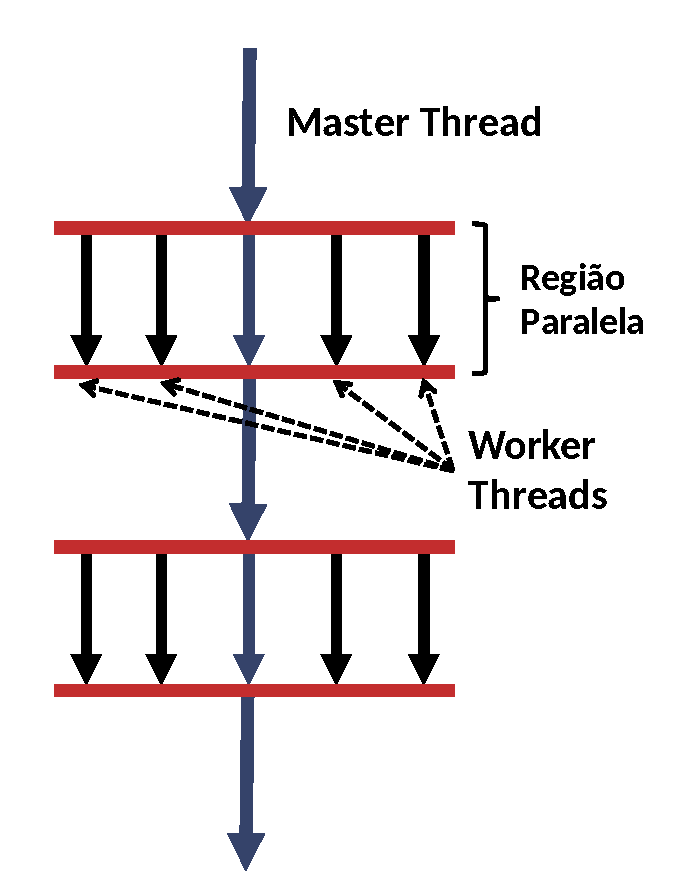
\includegraphics[width=0.4\textwidth]{figs/forkjoin.pdf} \\
    Fonte: desenvolvido pelo autor.
	\label{fig:forkjoin}
\end{figure}

Por meio de diretivas de compilação é possível definir o comportamento do
OpenMP, inclusive, determinar regiões paralelas e outras funções da \api.
O Código~\ref{cod:exemplo-openmp} apresenta um exemplo de uma função
que implementa o produto escalar entre dois vetores (\texttt{a} e \texttt{b}) paralelizada
com uso do OpenMP. A região paralela é criada pela diretiva de compilação
\texttt{\#pragma omp parallel} (linha 5). Variáveis dentro de uma região paralela
podem ser classificadas como \texttt{shared} (compartilhadas) ou \texttt{private} (privadas),
possibilitando assim o gerenciamento da execução pela \api. Uma variável marcada como \texttt{shared}
é compartilhada entre as \textit{threads} de uma região paralela. Por outro lado, variáveis marcadas
como \texttt{private} são privadas para cada \textit{thread}, isto é, cada \textit{thread} possuirá uma
cópia privada da variável. Desta forma, as modificações sobre elas serão feitas localmente em cada
\textit{thread}.

As diretivas do OpenMP, além de determinar regiões paralelas, possibilitam
paralelizar \textit{loops} de maneira automática, onde as iterações
do \textit{loop} são distribuídas, de forma automática e flexível, sobre as
\textit{threads} da região paralela. A paralelização das iterações do \textit{loop} é mostrada na linha 6 do
Código~\ref{cod:exemplo-openmp} com uso da cláusula \texttt{for}. Além disso, operações de redução podem ser
utilizadas ao fim de uma região paralela, aplicando sobre uma variável a
operação especificada. Ao final da região paralela, o resultado é atribuído a uma variável compartilhada. A redução
é necessária no caso do produto escalar mostrado no Código~\ref{cod:exemplo-openmp}, sendo necessário
utilizar a cláusula \texttt{reduction} sobre a variável \texttt{prod}. A operação de redução utilizada no caso do produto
escalar é a soma (\texttt{+}).

\begin{figure}[t]
	\begin{lstlisting}[
		caption=Produto escalar paralelo com OpenMP.,
		label=cod:exemplo-openmp,
	]
	int produto_escalar(int *a, int *b, int tamanho)
	{
		int prod = 0;

		#pragma omp parallel for private(i) shared(a, b) \
                                        reduction(+:prod)
		for (int i = 0; i < tamanho; i++)
			prod += a[i] * b[i];

		return(prod);
	}
	\end{lstlisting}
\end{figure}

Devido à abstração que o modelo oferece, poucas modificações de código são
necessárias para paralelizar uma aplicação. \posix \textit{threads} é outro
modelo que pode ser utilizado, contudo com uma menor abstração que o modelo
OpenMP.

%Computação paralela em uma arquitetura multiprocessada contém diversas
%dificuldades para o desenvolvimento de código, como: \textbf{(i) dependência de
%    dados:} quando um processo ou \textit{thread} está executando uma parte do
%código, outra \textit{thread} deve ter os dados atualizados corretamente. Esta
%dependência pode gerar problemas, como \textit{deadlocks} e \textit{livelocks}.
%\textit{Deadlocks} são conflitos que ocorrem entre \textit{threads}, quando uma
%\textit{thread} $A$ precisa de um recurso alocado por uma \textit{thread} $B$
%que, por sua vez, precisa de um recurso alocado pela \textit{thread} $A$, ocorre
%um ciclo na execução, caracterizando um \textit{deadlock}. Por outro lado,
%\textit{Livelocks} são similares aos \textit{deadlocks}, contudo o estado das
%\textit{threads} estão em constante mudança, fazendo com que nenhum deles
%continue sua execução normalmente, pois a cada mudança um \textit{deadlock}
%ocorre. Além disso, dependências geram problemas de sincronização entre
%\textit{threads}, deixando para o desenvolvedor da aplicação a tarefa de
%gerenciar corretamente a execução. \textbf{(ii) Condição de Corrida:} uma
%\textit{thread} escreve sobre uma váriavel ou, mais especificamente, um espaço
%de memória, enquanto outra \textit{thread} fará alguma operação sobre esse mesmo
%espaço. Isso pode gerar inconsistências de dados, entre outros problemas.

\subsection{MPI}

% \todo[inline]{
% - Motivação para usar MPI:
%
% A programação paralela em multicomputadores é feita através da utilização de múltiplos processos que se comunicam
% através de trocas de mensagens. Devido à característica de baixo nível intrínseca do modelo de troca de
% mensagens, utilizar \textit{sockets} manualmente para a comunicação entre nós de
% uma rede de \textit{clusters} é inadequada para o desenvolvedor. Portanto, mostra-se necessário utilizar
% APIs de mais alto nível, possibilitando uma maior abstração ao desenvolvedor.
% }
%
% \todo[inline]{
% - Dizer que MPI é a API mais amplamente utilizada para programação paralela em multicomputadores, ou seja, para arquiteturas multicomputadas, ou seja, com memória distribuída.
% }
%
% \todo[inline]{
% - Apresentar as principais ideias do MPI: processos MPI, rank, Send/Recv, comunicações coletivas, ...
% }

A programação paralela em multicomputadores é feita através da utilização de múltiplos processos que se comunicam
através de trocas de mensagens. Devido à característica de baixo nível intrínseca do modelo de troca de
mensagens, utilizar \textit{sockets} manualmente para a comunicação entre nós de
uma rede de \textit{clusters} é inadequada para o desenvolvedor. Portanto, mostra-se necessário utilizar
APIs de mais alto nível, possibilitando uma maior abstração ao desenvolvedor.

O \mpi é uma \api utilizada amplamente em multicomputadores fornecendo uma maior
abstração em relação à programação sobre \textit{sockets}. A \api é baseada no
modelo \spmd, onde todos os processos executam o mesmo programa, porém cada processo é responsável
por realizar computações em dados distintos.

A \api fornece diversas funções aos desenvolvedores. A função \texttt{MPI\_Init()} permite inicializar o ambiente \mpi.
Após a inicialização, cada processo \mpi possuirá um identificador único (de $0$ até $np-1$, onde $np$ é o número total
de processos \mpi em execução). Esse identificador único, denominado \textit{rank}, poderá ser utilizado em conjunto com
instruções de seleção (\texttt{if-else}) para determinar que processos \mpi
distintos possam executar códigos distintos. Além disso,
ele será utilizado nas primitivas de comunicação do \mpi para especificar os remetentes e destinatários das mensagens.
Para finalizar o ambiente \mpi é feita uma chamada para a função \texttt{MPI\_Finalize()}. O envio de mensagens
é realizado pela função \texttt{MPI\_Send()}, que construirá a mensagem, e irá
adicionar o \textit{rank} do destinatário, o \textit{rank} do remetente, entre
outras informações. A função \texttt{MPI\_Recv()} será responsável por receber a
mensagem enviada pelo processo, e irá armazená-la no espaço de memória
do processo destinatário.

O Código~\ref{cod:exemplo-mpi} mostra um exemplo de um programa em \mpi. Nesse
exemplo, o processo com \textit{rank} igual a zero
envia uma mensagem a todos os demais processos. Ao receber a mensagem, cada um dos demais processos imprime na tela a mensagem
recebida. As funções \texttt{MPI\_Comm\_rank()} e \texttt{MPI\_Comm\_size()} são utilizadas para armazenar nas variáveis \texttt{rank} e \texttt{size}
o \textit{rank} do processo e o número total de processos, respectivamente. Nas
linhas 12-13, o processo com \textit{rank} igual a zero envia para os
demais processos a mensagem \texttt{``Ola mundo!''}. As linhas 16-19 são executadas somente pelos demais processos, onde cada processo
realiza o recebimento da mensagem e a imprime na tela juntamente com seu \textit{rank}.

\begin{figure}[t]
	\begin{lstlisting}[
		caption=Exemplo de um programa MPI.,
		label=cod:exemplo-mpi,
	]
	int main(int argc, char **argv)
	{
		int rank, size;

		MPI_Init(argc, argv);

		MPI_Comm_rank(MPI_COMM_WORLD, &rank);
		MPI_Comm_size(MPI_COMM_WORLD, &size);

		if (rank == 0) {
			char mensagem[11] = "Ola mundo!";
			for (int i = 1; i < size; i++)
				MPI_Send(&mensagem, 11, MPI_CHAR, i, 0, MPI_COMM_WORLD);
		}
		else {
			char mensagem[11];
			MPI_Recv(&mensagem, 11, MPI_CHAR, 0, MPI_ANY_TAG,
                             MPI_COMM_WORLD, MPI_STATUS_IGNORE);
			printf("Processo %d recebeu: %s\n", rank, mensagem);
		}

		MPI_Finalize();
		return(0);
	}
	\end{lstlisting}
\end{figure}

Além de comunicações do tipo ponto-a-ponto, existem comunicações coletivas e de sincronização entre
todos os processos. A função \texttt{MPI\_Barrier()} é uma barreira de sincronização, responsável por bloquear a
execução de um processo até que todos os outros processos cheguem na barreira.
Por outro lado, a função \texttt{MPI\_Bcast()} é responsável por enviar a mesma
mensagem de um processo para todos os outros processos do sistema de forma otimizada.

%
% \renewcommand{\lstlistingname}{Código}
% \definecolor{lightgray}{rgb}{0.97,0.97,0.97}
% \definecolor{lightred}{rgb}{1,0.7,0.7}
%
% \lstdefinelanguage{cc}{
%     language     = C++,
%     morekeywords = {Array2D, __parallel__, Mask2D, Stencil2D, pragma, omp, parallel, printf},
% }
%
% \lstset{
% numbers=none,
% stepnumber=1,
% numbersep=-8pt,
% numberstyle=\small\color{black},
% basicstyle=\scriptsize\ttfamily,
% keywordstyle=\color{blue},
% commentstyle=\color{black},
% stringstyle=\color{black},
% numberstyle=\footnotesize\ttfamily\color{black},
% escapeinside={(@}{@)},
% frame=none, %single
% tabsize=2,
% float,
% language=cc, %morecomment=[l][{\color[rgb]{0.1, 0.2, 0.8}}]{},
% %aboveskip=0.1in, % space before the caption
% %belowskip=0.1in, % space after listing
% captionpos=b,
% showstringspaces=false,
% %belowcaptionskip=1\baselineskip,
% %breaklines=true,
% %moredelim=[l][\color{blue}]{\#pragma},
% backgroundcolor=\color{white},
% %xleftmargin=.2\textwidth, xrightmargin=.2\textwidth
% }
%
% \begin{figure}[thp] % the figure provides the caption
% \centering          % which should be centered
% \begin{tabular}{c}
%
% \begin{lstlisting}[]
%     (@\textcolor{blue}{\#}@)pragma omp parallel
%     printf("Hello World!");
% \end{lstlisting}
% \end{tabular}
% \caption*{Exemplo de código OpenMP.}
% \end{figure}
%
% \todo{Apresentar código \MPI}


%Ao aperfeiçoar esses modelos, começaram a surgir processadores para \hpc com
%vários \textit{cores} de processamento. Esses processadores utilizam várias
%técnicas, que abordam o paralelismo e características específicas de cada
%máquina, para aumentar o desempenho de aplicações. Com o aumento da importância
%do consumo de energia, novos porcessadores \textit{manycore} de baixo consumo de
%energia começaram a surgir. Contudo, processadores \textit{manycore} são
%onerosos e suceptíveis à erros, apresentando diversos problemas para o
%desenvolvedor~\cite{pereira15}. Geralmente, núcleos de processamento sem
%coerência de \textit{cache} são distribuídos em uma arquitetura organizada em
%\textit{clusters}, onde cada \textit{cluster} possui uma memória local
%(compartilhada somente entre os \textit{cores} do \textit{cluster}). Dessa
%forma, a comunicação entre \textit{clusters} deve ser feita de uma forma
%distribuída e a comunicação intra-\textit{cluster} deve ser feita por meio do
%modelo de memória compartilhada. Devido à comunicação entre os \textit{clusters}
%o peso do tempo de comunicação pode ter um grande impacto no tempo total de
%execução.
%-------------------------------------------------------------------

\subsection{Modelo de Programação do MPPA-256}
\label{sec:prog-mppa}
% \todo[inline]{
% - Falar de como se programa o MPPA: processo mestre roda no I/O, ele faz spawn de um
% processo escravo para cada cluster, cada processo escravo pode criar até 16 threads.
% }
%
% \todo[inline]{
% - Threads podem ser criadas usando POSIX ou OpenMP (que foi tratado anteriormente)
% }
%
% \todo[inline]{
% - Explicar que MPPA não tem suporte para a API MPI. Portanto, é necessário utilizar uma API de comunicação low-level
% desenvolvida pela Kalray. Explicar que cada  cluster tem seu espaço de endereçamento, que se usa o conceito de portais, para se
% fazer escrita remota, etc... Falar um pouco de como funciona essas comunicações através da NoC.
% }
%
% \todo[inline]{
% - Finaliza falando das dificuldades de se programar com essa API low-level (texto abaixo):
% }

O \mppa possui uma arquitetura interessante que permite a execução de aplicações paralelas
que seguem um modelo \textit{mestre/escravo}. Nesse modelo, o processo \textit{mestre} é responsável
pela coordenação e pela divisão das tarefas entre os processos \textit{escravos}. Os processos \textit{escravos},
por outro lado, são responsáveis por receber tarefas e computá-las, devolvendo os resultados para o processo
mestre. No \mppa, o processo mestre é executado em um \rman no subsistema de
\es, e é responsável por inicializar os processos escravos. Cada processo escravo
é executado em um \textit{cluster} distinto, podendo criar até 16 \textit{threads} \posix, uma para cada \pe.

A Figura~\ref{fig:MPPAIPCTutorial} ilustra o funcionamento do modelo mestre/escravo
no \mppa. O processo mestre será responsável por iniciar os
\textit{clusters} por meio da função \texttt{MPPA\_Spawn()}.
O \mppa não possui suporte para o \mpi, desta forma, os processos mestre e
escravos utilizam objetos de comunicação, como portais e filas, de
uma \api proprietária de baixo nível do \mppa, similar à \posix \ipc.

Cada processo escravo possui um espaço de endereçamento distinto, desta forma,
são utilizados portais para efetuar a comunicação entre o mestre e os escravos, e entre escravos. Os
portais efetuam escrita e leitura remota, onde um processo deve criar um portal
com uma classificação, denominada \textit{tag}, e relacionar o portal com um
espaço de endereçamento para realizar a comunicação.

Para efetuar a escrita em um espaço de endereçamento é necessário chamar uma
função denominada \texttt{mppa\_pwrite()}. Essa função possui como parâmetros o
portal que será utilizado na comunicação e o tamanho do dado que será enviado.
A função \texttt{mppa\_aio\_read()} realizará a leitura dos dados recebidos pelo
portal, relacionando o portal responsável pela leitura com o espaço de
endereçamento em que o dado será armazenado.

\begin{figure}
	\centering
	\caption{Esquemático do modelo mestre/escravo no \mppa.}
	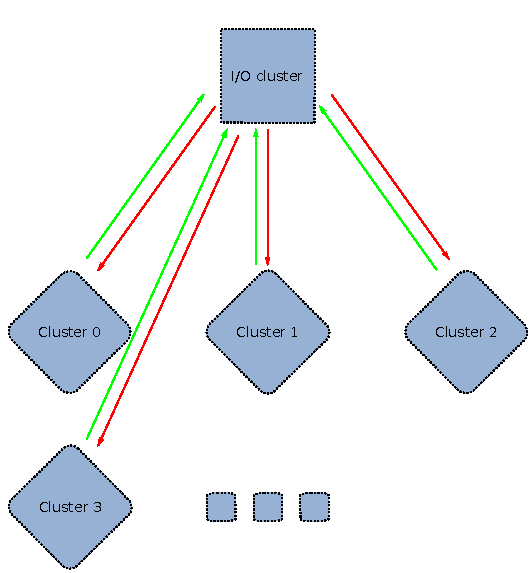
\includegraphics[width=0.5\textwidth]{figs/MPPAIPCTutorial.pdf} \\
    Fonte: Manual do \mppa.
	\label{fig:MPPAIPCTutorial}
\end{figure}

Um programa para o \mppa é composto por, pelo menos, dois arquivos principais:
um deles conterá o código a ser executado pelo processo o mestre e outro conterá o código
a ser executado por cada processo escravo. Esses arquivos são compilados separadamente,
gerando dois arquivos binários (um para o processo mestre e outro para os processos escravos).
O binário dos escravos é utilizado como argumento de entrada da função \texttt{MPPA\_Spawn()}
descrita anteriormente durante a criação dos processos escravos.

Trabalhos anteriores mostraram que desenvolver aplicações paralelas otimizadas
para o \mppa é um grande desafio~\cite{Castro-IA3-JPDC:2014} devido a alguns
fatores importantes. O primeiro deles está relacionado ao \textbf{modelo de
    programação híbrido} exigido pelo processador: \textit{threads} em um mesmo
\textit{cluster} se comunicam através de uma memória compartilhada local, porém
a comunicação entre \textit{clusters} é feita explicitamente via \noc, em um
modelo de memória distribuída. Mais especificamente, aplicações desenvolvidas
para o \mppa precisam utilizar duas bibliotecas de programação paralela para
utilizar os recursos do processador: OpenMP, baseado em um modelo de memória
compartilhada, utilizada para paralelizar a computação dentro de cada
\textit{cluster} e a \api proprietária do \mppa, que segue um modelo de memória
distribuída, sendo utilizado na comunicação entre os \textit{clusters} e o
subsistema de \es por meio da \noc. O segundo fator importante está relacionado
à \textbf{capacidade limitada de memória} no \textit{chip}: cada \textit{cluster}
possui apenas 2~\mb de memória local de baixa latência. Portanto, aplicações
reais precisam constantemente realizar comunicações com o subsistema de \es
conectado à memória \lpddr. Por fim, o último fator está diretamente relacionado
à \textbf{ausência de coerência de \textit{cache}}: cada \pe possui uma memória
\textit{cache} privada sem coerência de \textit{cache}, sendo necessário o uso
explícito de instruções do tipo \textit{flush} para atualizar a \textit{cache}
de um \pe quando necessário.


\begin{figure}[t]
	\centering
	\caption{Ilustração do padrão \stencil.}
	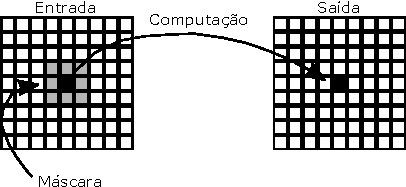
\includegraphics[width=0.6\textwidth]{figs/stencilComp.pdf} \\
    Fonte: desenvolvido pelo autor.
	\label{fig:stencil}
\end{figure}

\section{O Padrão \textit{Stencil}}
\label{sec:stencil}

As dificuldades na computação paralela tem um grande impacto no desenvolvimento de aplicações. Com o
desenvolvimento de aplicações paralelas, começou-se a notar um padrão entre
elas. Com isso, foram criados os padrões paralelos para simplificar o
desenvolvimento de código.
% ~\cite{Cole M. Algorithmic skeletons: structured management of parallel computations, Research monographs in parallel and distributed computing.
% London: Pitman; 1989.}
% McCool MD. Structured parallel programming with deterministic patterns. Proceedings of the 2Nd USENIX Conference on Hot Topics in Parallelism, HotPar'10, USENIX Association, Berkeley, CA, 2010; 5–5.
Para uma maior abstração e redução da complexidade dos padrões, foram propostos
esqueletos paralelos (\textit{skeletons}). Na programação paralela com esqueletos, o esqueleto é responsável por
gerenciar o controle de tarefas e dados, retirando essa responsabilidade do
desenvolvedor. Desta forma, é possível simplificar grande parte do
desenvolvimento de aplicações paralelas e auxiliar em outras funções que podem
trazer uma maior dificuldade ao desenvolvedor. Mais especificamente, o
desenvolvedor irá focar apenas em especificar o algoritmo, deixando o esqueleto
gerenciar os detalhes de execução, diminuindo o tempo de desenvolvimento e
\textit{debug} da aplicação.

Existem diversos padrões paralelos, como o \textit{map}, \textit{reduce},
\textit{scan}, \stencil, entre outros. Dentre os padrões existentes, o
padrão \stencil é de grande importância tanto no ambiente acadêmico quanto no
industrial, utilizado em diversos campos importantes, como física quântica,
previsão do tempo e processamento de imagens~\cite{pereira15}.

\begin{figure}[t]
	\begin{lstlisting}[
		caption=Exemplo de código \stencil (aplicação Jacobi).,
		label=cod:exemplo-stencil,
	]
	void jacobi(int tsteps, int N, float *A, float *B){
		int t, i, j;
		float c1 = 0.2;

		for (t = 0; t < tsteps; t++){
			for (i = 1; i < N-1; i++)
				for (j = 1; j < N-1; j++)
					B[i,j] = c1 * (A[i,j] + A[i,j-1] + A[i,j+1] + A[i+1,j]
                         + A[i-1,j]);

			for (i = 1; i < N-1; i++)
				for (j = 1; j < N-1; j++)
					A[i,j] = B[i,j]
		}
	}
\end{lstlisting}
\end{figure}

O padrão \stencil atualiza elementos de uma matriz de entrada ($A$),
de acordo com um padrão especificado. Mais especificamente, em uma aplicação
\stencil, cada iteração utiliza a máscara de vizinhança responsável por determinar os vizinhos
utilizados na computação. A máscara é aplicada sobre $A$ para determinar o valor de cada
célula da matriz de saída ($B$). No exemplo da Figura~\ref{fig:stencil}, o
valor de cada célula da matriz de saída é determinado em função dos
valores de cada uma das células vizinhas adjacentes da matriz de entrada. Esse processo é realizado
para todas as células da matriz de entrada, produzindo uma matriz de saída contendo o resultado da computação \stencil. Além disso, o padrão possibilita a computação
iterativa, isto é, ao final de uma iteração, a matriz de saída será
considerada como a matriz de entrada para a próxima iteração,
caracterizando uma nova iteração da computação.

O Código~\ref{cod:exemplo-stencil} apresenta um exemplo do código de uma aplicação baseada no padrão
\stencil, cujo o objetivo é a realização da resolução de equações matriciais pelo método iterativo de Jacobi.
O número de iterações é determinado pelo parâmetro \texttt{tsteps} (linha 5). A computação
\stencil é realizada lendo-se as informações da matriz de entrada \texttt{A} e escrevendo-se os resultados em uma matriz de saída \texttt{B}, ambas de tamanho \texttt{N*N}.
Nesse exemplo, foi utilizado um coeficiente \texttt{c1} e uma vizinhança de 5 elementos (linha 8). A vizinhança de 5 elementos
representa a célula central e as 4 células adjacentes à célula central (cima, baixo, esquerda e direita).
Devido à característica iterativa desta aplicação, existe uma troca de dados entre as matrizes \texttt{A} e \texttt{B}
(linhas 10-12) para que o resultado da iteração \texttt{i} possa ser utilizado como entrada na iteração
\texttt{i+1}.

% \todo[inline]{- Adicionar 1 ou 2 parágrafos falando de exemplos de aplicações que usam esse padrão.
% Podes usar o Fur e o Jacobi.}

\section{PSkel}
\label{sec:pskel}

O \pskel é um \fw de programação em alto nível para o padrão \stencil, que
oferece suporte a execuções paralelas em arquiteturas heterogêneas incluindo \cpu
e \gpu. Utilizando uma única interface de programação escrita em C++, o usuário é
responsável por definir o \textit{kernel} principal da computação \stencil,
enquanto o \fw se encarrega de gerar código executável para as diferentes
plataformas paralelas e realizar todo o gerenciamento de memória e transferência
de dados entre dispositivos de forma transparente~\cite{pereira15}. Mais
especificamente, o \pskel traduz as abstrações em código C++ de baixo nível,
compatível com Intel TBB e NVDIA CUDA.

A \api do PSkel possibilita a definição de \textit{templates} para a manipulação
de estruturas $n$-dimensionais, denominadas \texttt{Array} (1 dimensão),
\texttt{Array2D} (2 dimensões) e \texttt{Array3D} (3 dimensões). Além disso, o
\fw provê abstrações para a definição da vizinhança do \stencil (\texttt{Mask})
e o \textit{kernel} da computação \stencil (\texttt{stencilKernel()}). O
\texttt{stencilKernel()} é um método a ser implementado pelo usuário que
descreve, especificamente, a computação que será executada para cada célula do
\texttt{Array} de entrada com base nos valores de sua vizinhança (\texttt{Mask}).

Desta forma, o desenvolvedor deverá seguir os seguintes passos para desenvolver
uma aplicação \stencil com \pskel:

\begin{enumerate}
	\item Identificar a dimensão do problema, construindo estruturas de acordo com
	os \textit{containers} especificados pelo \fw;

	\item Definir o método \texttt{stencilKernel()} que descreve a computação executada
	sobre os elementos da máscara e do \texttt{Array} de entrada;

	\item Instanciar um ou mais objetos \texttt{Stencil} para gerenciar os encapsulamentos,
	alocação de memória e chamadas para efetuar a computação determinada pelo método
	\texttt{stencilKernel()}. Mais especificamente, os \textit{containers} são estruturas que
	armazenam \texttt{Arrays} para leitura/escrita de dados. Eles são responsáveis por
	gerenciar a alocação de memória na \cpu e \gpu de maneira transparente.

	\item Instanciar a classe de \textit{Runtime} que adota um padrão \textit{Facade} que
	efetua a abstração dos detalhes da implementação e configurações do padrão \stencil.
	Essa classe provê os métodos de execução para os padrões \stencil, além do
	particionamento transparente de tarefas e dados entre \cpu e \gpu.
\end{enumerate}

% \begin{figure}[t]
% \centering
% 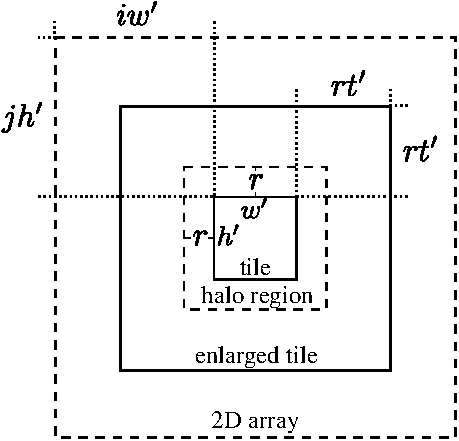
\includegraphics[width=0.3\columnwidth]{figs/tile.pdf}
% \caption{ Diagrama do \textit{tiling} 2D. Um \textit{tile} lógico (linha interna sólida) é contido dentro do Array
%     2D (linha externa pontilhada) com \textit{offsets} verticais e horizontais dado por $j  h^\prime$
%     e $i  w^\prime$. Computar $t^\prime$ consecutivas iterações estêncil no \textit{tile} requer um aumento no
%     \textit{tile} lógico com uma \textit{ghost zone} (área entre a linha interna sólida e a linha externa sólida), que é constituída
%     de regiões \textit{halo} (área entre a linha interna sólida e a linha interna pontilhada).}
% \label{fig:gputile}
% %\vspace{-4em}
% \end{figure}
%

\begin{figure}[t]
	\begin{lstlisting}[
		caption=Exemplo do código da aplicação Jacobi no PSkel.,
		label=cod:exemplo-pskel,
	]
	__parallel__ void
	stencilKernel(Array2D<float> A, Array2D<float> B, Mask2D<int> mask,
								struct Arguments args, int x, int y){
		B(x,y) = args.alpha * (A(x,y+1) + A(x,y-1) + A(x+1,y)
                           + A(x-1,y));
	}

	int main(int argc, char **argv) {
		/* declaracoes de variaveis omitidas */

		Array2D<float> input(A, M, N);
		Array2D<float> output(B, M, N);
		int neighbors = {{0,1}, {-1,0}, {1,0}, {-1,0}};
		Mask2D<int> mask(4, neighbors);
		struct Arguments args(alpha);

		Stencil2D<Array2D<float>, Mask2D<int>, Arguments>
			jacobi(A, B, args);
		jacobi.runIterative(device::GPU, tsteps, 1.0);

		return(0);
	}
\end{lstlisting}
\end{figure}

Em uma aplicação \stencil iterativa, cada iteração utiliza a máscara de
vizinhança (\texttt{Mask}) sobre o \texttt{Array} de entrada para determinar o
valor de cada célula do \texttt{Array} de saída. No exemplo da
Figura~\ref{fig:stencil}, o valor de cada célula do \texttt{Array} de saída é
determinado em função dos valores de cada uma das células vizinhas adjacentes.
Esse processo é realizado para todas as células do \texttt{Array} de entrada,
produzindo um \texttt{Array} de saída da computação \textit{stencil}. Ao final de uma
iteração, o \texttt{Array} de saída será considerado como \texttt{Array} de
entrada para a próxima iteração no caso de uma aplicação \textit{stencil} iterativa.

O Código~\ref{cod:exemplo-pskel} apresenta um exemplo da aplicação Jacobi discutida na
Seção~\ref{sec:stencil} (Código~\ref{cod:exemplo-stencil}), porém agora implementada no \fw \pskel.
Nesse exemplo, a função \stencil principal da aplicação está implementada no método \texttt{stencilKernel()} nas linhas 1-5.
As estruturas para efetuar a computação, como o \texttt{Array} de entrada (\texttt{input}) e de saída (\texttt{output}), são mostrados nas linhas 10-11.
O formato da vizinhança é especificado na linha 12, sendo guardado na variável \texttt{neighbors}.
Então, a máscara é construída na linha 13 com base na vizinhança definida anteriormente.
Estruturas como \texttt{Array2D}, \texttt{Mask2D}, são exemplos dos
\textit{containers} disponibilizados pelo \fw. A classe de \textit{runtime} é
determinada pela estrutura \texttt{Stencil2D} (linha 16), onde ao efetuar a chamada para
função \texttt{runIterative()} (linha 18), a execução da computação irá iniciar.

% \todo[inline]{Falar mais precisamente o que é feito em cada linha.}

É possível notar que o \textit{kernel} da computação \stencil (linha 4) fica mais simplificado em relação ao
código original do Jacobi mostrado anteriormente (Código~\ref{cod:exemplo-stencil}), pois as iterações da aplicação
(\texttt{tsteps}) e os \textit{loops} de computação sobre as matrizes ficam implícitos, sendo
gerenciados pelo \fw. Os elementos das matrizes são determinados pelos
parâmetros \texttt{x} e \texttt{y} da função \texttt{stencilKernel()}. Além disso, o coeficiente
da aplicação Jacobi é passado como parâmetro por uma \texttt{struct} denominada
\texttt{Arguments} (linha 14).



\chapter{Trabalhos Relacionados}

A proposta deste trabalho está diretamente relacionada a diversos outros trabalhos de pesquisa.
A seguir, serão citados alguns trabalhos de pesquisa que fazem uso de esqueletos paralelos em
arquiteturas \textit{manycore}. Além disso, serão destacados alguns trabalhos de pesquisa sobre
o \mppa.

% \todo[inline]{Aqui, acho que poderia subdividir os trabalhos relacionados em subseções, de acordo com os assuntos que eles tratam.}

\subsection{Esqueletos paralelos e padrão \textit{stencil}}
\emph{Buono}~\etal~\cite{buono13} portaram um \fw baseado em esqueletos paralelos,
chamado de \emph{FastFlow}, para o processador \textit{manycore} \emph{TilePro64}.
Esse processador possui 64 núcleos de processamento idênticos, interconectados
por uma malha da \noc. O \fw \emph{FastFlow} provê padrões de \textit{design}
customizáveis, como, por exemplo, \textit{pipelines} e \textit{task farms},
que podem ser compostas para formar outros esqueletos, como \textit{map} e
\textit{reduce}.

De forma similar, \emph{Thorarensen}~\etal~\cite{thoraransen16} apresentaram um
novo \textit{back-end} do \fw \emph{SkePU} para o processador \textit{manycore}
de baixa potência \emph{Myriad2}. Esse processador possui uma arquitetura
heterogênea, tendo como alvo dispositivos com limites em questão de energia.
O \fw \emph{SkePU} provê uma interface de programação para esqueletos paralelos
como o \textit{map}, \textit{reduce}, e \textit{stencil}, com suporte para
diferentes \textit{back-ends}, incluindo processadores multicores e \gpus.

%------Trabalho relacionado sobre técnicas de tiling sobre o padrão estêncil.
%------Deixar para mencionar sobre trabalhos relacionados à isso.
\emph{Lutz}~\etal~\cite{lutz13} utilizaram técnicas de \textit{tiling} em
computações \textit{stencil} para lidar com a capacidade limitada de memória
de \gpus em ambientes multi-\gpu, utilizando as memórias das \gpus
coletivamente. De forma similar, \emph{Gysi}~\etal~\cite{gysi15} propuseram um \fw
para otimizações automáticas de \textit{tiling} em computações \textit{stencil}
situadas em um ambiente híbrido \cpu{}-\gpu.

%------------------------------------------

\subsection{Processadores \textit{manycore} de baixo consumo de energia}
Alguns trabalhos surgiram recentemente com intuito de avaliar o uso de
processadores \emph{manycore} em CAD, além de discutir os desafios do
desenvolvimento de aplicações para esses processadores.
Em~\cite{SCCEnergy:2012}, os autores compararam o desempenho e o consumo
energético de um processador \emph{manycore} experimental da Intel denominado
\emph{Single-Chip Cloud Computer} (SCC) com outros tipos de processadores e
GPUs. Para realizar essa análise, os autores utilizaram um conjunto de
aplicações paralelas implementadas em Charm++~\cite{Charm:2012}. Os resultados
obtidos com o Intel SCC mostraram que \emph{manycores} são uma alternativa
viável, apresentando bom desempenho e baixo consumo energético.
Em~\cite{MPPA-1:2013}, os autores avaliaram o desempenho do processador
\emph{manycore} MPPA-256 no contexto de aplicações de decodificação de vídeo. Os
resultados mostraram que o desempenho do MPPA-256 é comparável ao desempenho de
processadores Intel atuais em uma decodificação de vídeo no padrão H.264,
consumindo 6 vezes menos energia.

Trabalhos recentes revelaram o desempenho e consumo energético do processador
MPPA-256, comparando-o a outros processadores \textit{multicore} de propósito
geral e embarcados, no contexto de diferentes aplicações
científicas~\cite{Castro-SBAC-PAD:2014,Castro-IA3:2013,Castro-IA3-JPDC:2014}. Os
resultados mostraram que o processador \emph{manycore} MPPA-256 apresenta em
alguns casos desempenho superior a processadores \emph{multicore} Intel Xeon 2.4
GHz com 8 \emph{cores}, além de um consumo de energia de até 13 vezes menor em
relação ao mesmo processador. Um outro trabalho recentemente publicado realizou
uma análise comparativa de desempenho e consumo de energia entre processadores
\emph{multicore} Intel de alto desempenho e ARM~\cite{Castro-Padoin-IET:2015}.
Os resultados mostraram que, apesar da potência dos processadores ARM ser pelo
menos 10 vezes menor que a dos processadores Intel de alto desempenho, o consumo
de energia nem sempre será melhor, sendo dependente das características da carga
de trabalho a ser executada.

\emph{Morari}~\etal~\cite{Valero:2012} propuseram uma implementação otimizada do
\textit{radix sort} para o processador \textit{manycore} Tilera TILEPro64. Os
resultados mostraram que a solução para o TILEPro64 provê uma melhor eficiência
energética em relação a um processador \textit{multicore} de propósito geral, como
o Intel Xeon W5590, e em relação a uma \gpu NVIDIA Tesla C2070.

Mais especificamente, \emph{Francesquini}~\etal~\cite{Castro-IA3-JPDC:2014} analisaram
três diferentes classes de aplicações (CPU-\textit{bound}, \textit{memory-bound}
e híbrida) usando plataformas paralelas, como o \mppa, e um multiprocessador \numa de
192 núcleos e 24 nós. Mostrou-se que arquiteturas \textit{manycore} podem ser muito
competitivas, mesmo se a aplicação é, naturalmente, irregular. Os resultados mostraram
que o \mppa pode obter um desempenho maior (e um consumo de energia menor) que um
processador \textit{multicore} de propósito geral (Intel Xeon E5-4640) em um ambiente
com cargas de trabalho variadas e \cpu{}-\textit{bound}. Todavia, em um ambiente com cargas
de trabalho \textit{memory-bound}, o processador \numa obteve um melhor desempenho
em relação ao \mppa, apesar de apresentar também um maior consumo de energia.
Entre as plataformas avaliadas, o \mppa apresentou a melhor eficiência
energética, reduzindo a energia consumida em aplicações \cpu{}-\textit{bound},
híbridas e \textit{memory-bound} em 6.9x, 6.5x e 3.8x, respectivamente.

% Trabalhos recentes que propuseram APIs e ambientes de execução para
% \emph{manycores}. Em~\cite{TSHMEM:2013}, os autores propuseram uma adaptação
% Espaço de Endereçamento Global Particionado (\emph{Partitioned Global Address
%     Space} -- PGAS) para simplificar o desenvolvimento de aplicações paralelas
% para os processadores \emph{manycore} TILE-Gx e TILEPro. Mais precisamente, os
% autores utilizaram a biblioteca OpenSHMEM como base para a proposta,
% utilizando-a como uma camada de abstração para as bibliotecas fornecidas pelo
% fabricante dos processadores. Com isso, aplicações atualmente implementadas
% utilizando a API OpenSHMEM podem ser executadas nos processadores
% \emph{manycore} da linha TILE sem que haja a necessidade de modificações no
% código.

\chapter{PSkel-MPPA}

Diversas dificuldades prejudicam o desenvolvimento de aplicações para
processadores \textit{manycore}, como o \mppa. Portanto, é interessante adaptar
o \fw PSkel para esse processador, trazendo as características de transparência
no particionamento de tarefas e dados para esse ambiente. Desta forma, o
desenvolvedor irá se preocupar apenas com o desenvolvimento da aplicação, e
utilizará dos benefícios que as características intrínsecas do processador
fornecem. Além disso, aplicações já desenvolvidas para o \fw serão portadas sem
alteração.

\chapter{Cronograma}
\label{cha:cronograma}
% \todo[inline]{Descrever resumidamente as atividades.}

Esta seção apresenta o cronograma de atividades proposto para a conclusão do projeto apresentado neste documento.
A Figura~\ref{fig:cronograma} apresenta o cronograma previsto, com atividades nomeadas de A1 até A7. A descrição de cada
uma dessas atividades é mostrada a seguir.

  \begin{figure}[ht]
    \begin{center}
	\resizebox{\textwidth}{!}{
             \begin{ganttchart}[
               x unit = 1cm,
               y unit title=0.4cm,
               y unit chart=0.6cm,
               hgrid,
               vgrid={{dotted, dotted, dotted, black}},
               title label font=\scriptsize,
               title/.append style={fill=gray!30},
               title height=1,
               bar/.append style={fill=gray!30,rounded corners=2pt},
               bar label font=\scriptsize,
               group label font=\scriptsize,
               ]{1}{16}
             	% \gantttitle{\textbf{2017}}{4}
                \gantttitle{\textbf{2018}}{16}\\
             	% \gantttitle{\textbf{Nov}}{2}
             	\gantttitle{\textbf{Dez}}{2}
        	 \gantttitle{\textbf{Jan}}{2}
        	 \gantttitle{\textbf{Fev}}{2}
        	 \gantttitle{\textbf{Mar}}{2}
        	 \gantttitle{\textbf{Abr}}{2}
        	 \gantttitle{\textbf{Mai}}{2}
        	 \gantttitle{\textbf{Jun}}{2}
        	 \gantttitle{\textbf{Jul}}{2} \\
        	 % \gantttitle{\textbf{Ago}}{2}
        	 % \gantttitle{\textbf{Set}}{2}
        	 % \gantttitle{\textbf{Out}}{2}
        	 % \gantttitle{\textbf{Nov}}{2}\\

             \ganttbar{A1}{1}{4} \\
             \ganttbar{A2}{3}{8} \\
             \ganttbar{A3}{7}{10} \\
             \ganttbar{A4}{8}{12} \\
             \ganttbar{A5}{13}{13} \\
             \ganttbar{A6}{14}{14} \\
             \ganttbar{A7}{15}{15}
             % \ganttbar{A8}{24}{24} \\
             % \ganttbar{A9}{25}{25} \\
             % \ganttbar{A10}{26}{26}
             \end{ganttchart}
     }
%  \end{adjustwidth}
     \caption{Cronograma de atividades.}\label{fig:cronograma}
  \end{center}
\end{figure}
% ---

\begin{itemize}
    \item \textbf{A1: Revisão aprofundada do estado da arte e prática.} Nesta etapa será
        realizada uma revisão mais aprofundada do estado da arte, buscando mais
        conteúdo sobre o tema da proposta, e uma base conceitual sobre abordagens de
        comunicação entre a \cpu e aceleradores.
    % \item \textbf{A2: Elaboração da proposta.} Nesta etapa será realizada a
        % elaboração da proposta
    \item \textbf{A2: Implementação da proposta.} Nesta etapa será realizada a
        implementação da proposta descrita no Capítulo~\ref{cha:proposta},
        buscando, também, estudar outras implementações para alcançar um bom
        desempenho e consumo de energia no processador \mppa.
    \item \textbf{A3: Realização de experimentos.} Nesta etapa serão realizados
        experimentos comparativos entre a implementação proposta sobre o \mppa e
        outros processadores. Os experimentos irão avaliar o desempenho e o consumo de
        energia da implementação proposta em relação à outros processadores.
    \item \textbf{A4: Escrita do rascunho do TCC II.} Nesta etapa será realizada
        a escrita do rascunho do TCC II, apresentando os experimentos desenvolvidos e a
        implementação completa da proposta.
    \item \textbf{A5: Preparação da defesa pública.} Nesta etapa será realizada
        a preparação de \textit{slides} e ensaio da defesa pública.
    \item \textbf{A6: Defesa pública.} Nesta etapa será realizada a defesa do
        projeto desenvolvido, mostrando os resultados obtidos e suas conclusões.
    \item \textbf{A7: Correções e entrega da versão final do TCC.} Nesta etapa
        será realizada as correções solicitadas pelos membros da banca, buscando
        melhorar a versão final do TCC.
\end{itemize}
% \begin{adjustwidth}{2.5cm}{}


\chapter{Conclusão}
\label{cha:conclusao}
% \todo[inline]{2 ou 3 parágrafos para concluir o que foi apresentado neste trabalho.}
Este trabalho discutiu inicialmente a relação entre o aumento de núcleos e o consumo de
energia nos processadores atuais. Como mostrado, a energia necessária para alcançar supercomputadores
\textit{Exascale} é muito alta, se tornando necessária a utilização de
novas técnicas e processadores energeticamente eficientes. Contudo, esses
processadores apresentam dificuldades de programação, trazendo problemas para o desenvolvimento
de aplicações e motivando a utilização de \fws sobre esses ambientes.

A adaptação do \fw para o processador \textit{manycore} \mppa é uma
tarefa desafiadora. Problemas de sincronização e comunicação deverão ser
tratados de forma especial, considerando a relação do tempo que o \fw gasta
comunicando e realizando a computação sobre os dados de entrada. Desta forma,
encontrar o melhor balanceamento entre o número de comunicações e a
quantidade de computação realizada \textit{clusters} é essencial.

Por fim, os experimentos realizados deverão abordar questões de desempenho e
energia, verificando a viabilidade da proposta em relação a outros
processadores.


% ----------------------------------------------------------
% Finaliza a parte no bookmark do PDF
% para que se inicie o bookmark na raiz
% e adiciona espaço de parte no Sumário
% ----------------------------------------------------------
% \phantompart

% ---
% Conclusão
% ---
%\chapter{Conclusão}
% ---

% ----------------------------------------------------------
% ELEMENTOS PÓS-TEXTUAIS
% ----------------------------------------------------------
% \postextual
% ----------------------------------------------------------

% ----------------------------------------------------------
% Referências bibliográficas
% ----------------------------------------------------------
\bibliographystyle{ufsc-alf}
\bibliography{bibliography}
% \addbibresource{bibliography.bib}
% \printbibliography

% ----------------------------------------------------------
% Glossário
% ----------------------------------------------------------
%
% Consulte o manual da classe abntex2 para orientações sobre o glossário.
%
%\glossary

%% ----------------------------------------------------------
% Apêndices
% ----------------------------------------------------------

% ---
% Inicia os apêndices
% ---
\begin{apendicesenv}

% Imprime uma página indicando o início dos apêndices
\partapendices

% ----------------------------------------------------------
\chapter{Quisque libero justo}
% ----------------------------------------------------------

\lipsum[50]

% ----------------------------------------------------------
\chapter{Nullam elementum urna vel imperdiet sodales elit ipsum pharetra ligula
ac pretium ante justo a nulla curabitur tristique arcu eu metus}
% ----------------------------------------------------------
\lipsum[55-57]

\end{apendicesenv}
% ---

%% ----------------------------------------------------------
% Anexos
% ----------------------------------------------------------

% ---
% Inicia os anexos
% ---
\begin{anexosenv}

% Imprime uma página indicando o início dos anexos
\partanexos

% ---
\chapter{Morbi ultrices rutrum lorem.}
% ---
\lipsum[30]

% ---
\chapter{Cras non urna sed feugiat cum sociis natoque penatibus et magnis dis
parturient montes nascetur ridiculus mus}
% ---

\lipsum[31]

% ---
\chapter{Fusce facilisis lacinia dui}
% ---

\lipsum[32]

\end{anexosenv}

%---------------------------------------------------------------------
% INDICE REMISSIVO
%---------------------------------------------------------------------
% \phantompart
% \printindex
%---------------------------------------------------------------------

\end{document}
